\documentclass[12pt]{article}

\usepackage[submission]{colm2025_conference}
\usepackage[utf8]{inputenc}
\usepackage{amsmath}
\usepackage{amssymb}
\usepackage{times}
\usepackage{url}
\usepackage{graphicx}
\graphicspath{{figures/}}
\usepackage{xcolor}
\usepackage{float}
\usepackage{booktabs}
\usepackage{enumitem}
\usepackage{setspace}
\usepackage{hyperref}
\hypersetup{colorlinks=true, linkcolor=blue, citecolor=blue, urlcolor=blue}

\doublespacing

\input{math_commands}

\newcommand{\pokeagent}{Pok\'{e}Agent}

\newcommand{\pokemon}{Pok\'{e}mon}

\newcommand{\tersoo}[1]{\textcolor{red}{#1}}

\usepackage{pifont}
\newcommand{\cmark}{\ding{51}}
\newcommand{\xmark}{\ding{55}}




\title{Can Vision-Language Models Become the Very Best? Agent Scaffolding and Self-Adaptive Methods for Embodied, Long-Horizon Play in \pokemon{} Emerald}


\begin{document}

\begin{center}
\maketitle
\textbf{Tersoo R.\ Upaa Jr.} \\
\vspace{1em}

With support from my advisor, Professor Chi Jin, and mentor Seth Karten \\ 
\vspace{1em}

Monday 13, April 2026
\vspace{2em}
\end{center}

% ============================================================================
% Chapter 1: Frontmatter (Pages 1-4 per ECE IW/Thesis Handbook)
% ============================================================================

% --- Page 1: Title page ---
% Title, author, date, and adviser are rendered by \maketitle in main.tex.
% The following statement is required by the ECE department.

\vspace{4em}
\begin{center}
Submitted in partial fulfillment\\ 
\vspace{1em}
of the requirements for the degree of\\
\vspace{1em}
Bachelor of Science in Engineering\\
\vspace{1em}
Department of Electrical and Computer Engineering\\
\vspace{1em}

Princeton University
\end{center}

\newpage

% --- Page 2: Declaration ---
\begin{center}
\vspace{5em}
I hereby declare that this Independent Work report\\ represents my own work in accordance with University\\ regulations.

\vspace{2em}

I hereby declare that this Independent Work report \\
does not include regulated human subjects research.

\vspace{2em}

I hereby declare that this Independent Work report \\ does not include regulated animal subjects research.

\vspace{2em}

\includegraphics[height=3em]{signature.png}\\
\noindent\rule{0.45\textwidth}{0.4pt}\\
\vspace{1em}
Tersoo R.\ Upaa Jr
\end{center}


\vspace{2em}



\newpage

% --- Page 3: Abstract ---

\begin{abstract}
We present three contributions toward evaluating and improving vision-language model (VLM) agents in long-horizon, embodied settings. First, we introduce the \pokeagent{} Challenge Speedrunning Benchmark, a standardized evaluation framework built on Pok\'{e}mon Emerald that requires agents to sustain coherent reasoning across thousands of sequential decisions under partial observability and real-time execution. Originating as a NeurIPS 2025 competition, the benchmark defines milestone-based metrics, supports both tutorial and extended evaluation settings, and provides the infrastructure for reproducible comparison of agent systems. Second, we develop an expert agentic harness ($\mathcal{H}_{\text{expert}}$) that decomposes gameplay into a multi-agent orchestration system with purpose-built subagents, hierarchical persistent memory, a runtime skill library, and sandboxed code execution. Tracing the harness through three stages of development---from a minimal competition-era scaffold through an intermediate design to the current expert system---we identify the architectural decisions that most impact long-horizon performance. Third, we introduce AutoEvolve, an algorithm that begins from a minimal harness ($\mathcal{H}_{\min}$) and iteratively modifies its own system prompt, subagents, memory, skills, and tools through in-context evolutionary optimization over trajectory segments, without environment resets. We evaluate all three harness configurations across tutorial and long-horizon settings using frontier VLMs and report results on milestone completion, wall-clock time, action efficiency, and cost. Our findings demonstrate that harness design is a first-order variable in agent performance and that automated harness discovery can approach expert-level scaffolding.
\end{abstract}

\vspace{1em}
\noindent\textbf{Keywords:} Long-horizon Evaluation, Speedrunning Benchmark, Vision-Language Model, AI System, Embodied Agent, Meta-Harness,

\newpage

% --- Page 4: Acknowledgments ---

\section*{Acknowledgments}

I would like to give a special thanks to Seth Karten for his extensive contributions towards this project and for his mentorship throughout my final year at Princeton. I've grown substantially in both technical ability and quality as a researcher through your guidance and support, in ways I could not have imagined a year ago; I am forever grateful.


To my family: thank you for your unwavering support throughout my time at Princeton and for encouraging me to pursue the things I care about, even when the path was not always clear. To my friends who tested early prototypes, endured my late-night debugging sessions, and reminded me that there is life outside the lab: this work is better because of you.

This project began as a simple question---can an AI agent play a game I grew up loving?---and grew into something far more ambitious than I could have anticipated. Working at the intersection of reinforcement learning, language models, and game AI has been the most rewarding intellectual experience of my undergraduate career, and I am grateful to everyone who helped make it possible.

Finally, I would like to thank SEAS and the ECE Department for their financial support.

\newpage

% --- Page 5: Table of Contents ---

\tableofcontents

\newpage

% --- Prelude ---

\section*{Prelude}

\textbf{[Personal prelude --- my history with Pok\'{e}mon (got pokemon black as a video game for christmas when I was nine years old, found community through showdown and competitive pokemon, what this project means to me personally, what I hope this project can mean for more people in the future... Who would've thought my love for Pokemon would so neatly intersect with a work that embodies four long years of learning, trial, growth, and becoming. ]}

\vspace{2em}
\noindent\rule{\textwidth}{0.4pt}

\newpage


% ============================================================================
% Section 1: Introduction (standalone)
% ============================================================================

\section{Introduction}\label{sec:introduction}

The study of Artificial Intelligence (AI) systems is undergoing a fundamental shift. Where language models were once evaluated on their ability to quickly produce fluent text in response to human prompts, the frontier has moved toward sustained, autonomous interaction within dynamic virtual and physical environments. AI systems are now expected to write and debug code across entire repositories, operate robotic platforms, and navigate virtual worlds, tasks that move beyond the demands of pretrained knowledge and extend towards the ability to plan, adapt, and progress over many hours of continuous execution.

Partial observability, long-horizon planning, and multi-modal perception are fundamental problems at the core of these emerging workflows. In these settings, agents are not only required to iterate on decisions that optimize for the successful completion of near-horizon tasks, but must also effectively plan for and maintain coherence across many thousands of environment interactions in pursuit of larger, often more abstract goals. In light of this new paradigm, there have been recent efforts to test the capabilities of frontier Large Language Models (LLMs) and the agent systems they underpin. Yet few existing benchmarks stress all three dimensions simultaneously under realistic conditions. Standard testbeds tend to isolate one axis: imperfect-information games emphasize equilibrium computation in short episodes, while open-ended environments test exploration but lack adversarial opponents or extended temporal commitments. As frontier language and vision-language models (VLMs) are increasingly deployed as autonomous agents, the gap between what existing benchmarks measure and what real-world autonomy demands has grown acute.

Pok\'{e}mon role-playing games (RPGs) offer a compelling case-study for this exact purpose. They combine a vast, partially observable state space with long-horizon, often non-linear narrative progression that demands thousands of cumulative decisions spanning exploration, resource management, combat, and spatial navigation. The recent surge of interest in Pok\'{e}mon-playing AI systems (Claude Plays Pok\'{e}mon~\citep{anthropic2025visible}, Gemini Plays Pok\'{e}mon~\citep{zhang2025geminiplayspokemon}, and GPT-5's completion of Pok\'{e}mon Red~\citep{engadget2025gptplayspokemon}) has demonstrated both the appeal of this domain and its limitations as a research vehicle. Fragmented across different games, harnesses, and evaluation criteria, the disconnected nature of these projects has made it difficult to rigorously disentangle both quantitative and qualitative metrics for success from the performance of the underlying model, sophistication of the harness architecture, or hardcoded assumptions about access to environment state.

This work addresses the fragmentation problem, advancing the state-of-the-art (SOTA) across three complementary dimensions. We first introduce an open \textbf{speedrunning benchmark}, as a robust foundation for evaluating frontier model and harness capabilities in long-duration, embodied settings and builds upon the testing framework established by the Speedrunning Track of the \pokeagent{} Challenge at NeurIPS 2025~\citep{karten2025pokeagent}. Our benchmark formalizes Pok\'{e}mon Emerald gameplay as a structured evaluation with standardized milestones, quantitative metrics, and infrastructure for fair cross-paradigm comparison. We have since extended it from the tutorial segment (through the first gym) to a long-horizon evaluation spanning many more segments of the game, where experiments proceed on the order of days and tens of thousands of environment interactions. Next, we present \textit{\pokeagent{},} a SOTA \textbf{custom VLM-agent harness} tasked with maintaining long-context coherence, developing and iterating upon plans, and effective problem solving across the Pok\'{e}mon Emerald storyline. Here, we detail the many insights spanning the development of \pokeagent{} from a simple four-module scaffold during the NeurIPS competition into a multi-agent system with abstractions for processing global session-level context, hierarchical memory management, skill-learning, subagent orchestration, and sandboxed code execution. We further compare PokeAgent against common CLI-agent harnesses (Claude Code, Codex CLI, Gemini CLI) revealing that, while coding-agent architectures are impressive out-of-the-box, they
nonetheless struggle to properly adapt to the unique set of constraints imposed by our speedrunning benchmark. Finally, we introduce \textbf{AutoEvolve}, a meta-harness framework and reset-free evolutionary algorithm designed to automate experiential learning by iteratively building agent scaffolding through in-context optimization over global trajectory segment history. Beginning from the simplest initialization, AutoEvolve seeks to bootstrap the development of its own harness by pruning and refining memories, distilling agent progress across entire episodes of environment interactions into skill and subagent abstractions, and refining system prompts accordingly with respect to the evolving harness. Unlike prior methods for model-level and agent self-adaptation that require full episodes and environment resets~\citep{agrawal2025gepa}, AutoEvolve operates in a fully online, reset-free manner, targeting continuous self-improvement in settings where environment resets are expensive or unfeasible. 

The remainder of this work is organized as follows. Chapter~\ref{sec:background} provides the necessary background, introducing relevant foundations in Markov Decision Processes, the Transformer architecture, reinforcement learning, and the Model Context Protocol, before surveying the broader motivation for this work. Chapter~\ref{sec:related_work} surveys related work across experiential learning, long-horizon benchmarks, embodied agents in RPG settings, and self-adaptive methods. Chapter~\ref{sec:formalization} formalizes our conception of \textbf{Embodied Agent Environments (EAEs)} and \textbf{Agentic Harnesses}, including a spectrum of harness configurations that frames the experimental comparisons in later chapters. Chapter~\ref{sec:benchmark} describes the speedrunning benchmark in detail: its environment design, evaluation criteria, and baselines. Chapter~\ref{sec:pokeagent} traces the development of the \pokeagent{} harness from its competition-era origins through its current multi-agent architecture, presenting early performance results that motivate our interest in automated harness evolution. Chapter~\ref{sec:autoevolve} presents AutoEvolve, including its methodology, experimental design across many agent-evaluation settings, and a discussion of our results. Chapter~\ref{sec:outlook} concludes with an exploration of the implications of this work and fruitful areas for future investigation across model distillation, ultra-long context (ULC) evaluations, and extensions to domains beyond Pok\'{e}mon.

\input{sections/ch2_background}
% ============================================================================
% Section 3: Related Work
% ============================================================================

\section{Related Work}\label{sec:related_work}

We survey several lines of research that inform the design of our benchmark, improvements made to our expert harness (\pokeagent{}), and AutoEvolve algorithm. These range from existing contributions to experiential learning, recursive language models, and various self-adaptive methods.

\subsection{Experiential Learning}\label{sec:experiential_learning}

A growing body of work explores how agents can accumulate and leverage experience over extended interactions, moving beyond static policy deployment toward systems that learn through interaction. While experiential learning has a deep tradition in the RL paradigm through self-play and policy optimization across episodes, experiential learning in the LLM setting emphasizes structured knowledge accumulation within and across sessions, using the model's own reasoning and reflection as the primary learning signal.

AriGraph~\citep{anokhin2024arigraph} constructs knowledge graph world models with episodic memory for LLM agents, enabling them to maintain structured representations of their environment across interactions. This approach addresses the inability of standard LLM agents to retain and organize discoveries, spatial relationships, and causal knowledge beyond the current context window. AriGraph demonstrates that persistent, structured memory can compensate for the finite context window and enable agents to more effectively reason over accumulated experience.

Language Models Meet World Models~\citep{xiang2023embodied} showed that grounding LLMs in embodied experience, rather than relying solely on pretraining knowledge, significantly improves their performance on downstream reasoning tasks. Their method finetunes on structured experiential data collected during embodied play, enabling agents to adapt to novel environments that diverge from their training distribution.

Recent work on in-context reinforcement learning (ICRL) has demonstrated that LLMs can perform implicit policy improvement from in-context reward signals~\citep{song2025icrl, karten2025economist}. We reason that if LMs can implicitly improve policies from reward signals presented in-context, then explicitly grounding these signals in the agent's trajectory and reflection process may further complement this capability. This principle informs several of the methods discussed in Chapter~\ref{sec:autoevolve}.

\subsection{Skill Learning}\label{sec:skill_learning}

A recurring theme in experiential learning is the curation of reusable behavioral skills. Voyager~\citep{wang2023voyager} demonstrated that language model agents can progressively acquire capabilities through interaction, storing successful programs in a growing code library indexed by natural language descriptions.

SkillRL~\citep{xia2026skillrl} provides a comprehensive treatment of this process. Rather than accumulating raw, often noisy and redundant trajectories, SkillRL introduces an experience-based distillation mechanism that extracts high-level behavioral patterns into a hierarchical skill library (SkillBank). An adaptive retrieval strategy enables the agent to access both general and task-specific heuristics at inference time, while a recursive evolution mechanism allows the skill library to co-evolve with the agent's policy during reinforcement learning training. On the ALFWorld, WebShop, and seven search-augmented benchmarks, SkillRL achieves state-of-the-art performance, outperforming strong baselines by over 15.3\% while significantly reducing the token footprint. The connections between SkillRL's distillation approach and our harness's skill-learning mechanism are revisited in Chapters~\ref{sec:pokeagent} and~\ref{sec:autoevolve}.

\subsection{Agent Memory}\label{sec:agent_memory}

Memory is the primary mechanism by which experiential learning persists beyond the immediate context window, and its design has emerged as a critical architectural decision for long-horizon agents. Agent memory systems generally organize knowledge along three axes: \emph{episodic memory} (logs of specific interactions and events), \emph{semantic memory} (accumulated facts, strategies, and world knowledge), and \emph{procedural memory} (learned skills and behavioral routines).

Generative Agents~\citep{park2023generative} introduced an influential memory architecture that combines recency, importance, and relevance-based retrieval to select which memories to surface during reasoning. This design enables believable long-term behavior in simulated social environments and has influenced subsequent work on agent memory, including retrieval-augmented approaches that treat memory as an external knowledge base to be queried at inference time.

MemGPT~\citep{packer2023memgpt} draws an explicit analogy between LLM context management and operating-system virtual memory. By implementing a hierarchical memory system with fast (in-context) and slow (external storage) tiers, MemGPT enables agents to intelligently move information in and out of their active context window, maintaining coherent behavior across interactions that would otherwise exceed context limits. This approach is particularly relevant to the long-context settings we consider, where the space of all possible information that might be relevant to an agent exceeds what can be reasonably stored at each step. Our expert harness leverages this hierarchical memory abstraction to efficiently store and dynamically access memory across all three axes.

\subsection{Recursive Language Models}\label{sec:rlm}

Recursive Language Models (RLMs)~\citep{zhang2025rlm} programmatically interact with and recurse over their own context. Rather than treating the context window as a passive repository of information, RLMs treat it as an active workspace that the model can read from, write to, and restructure. RLMs are particularly relevant to the problem of \emph{context rot}, where LMs experience a degradation in coherent reasoning as context windows grow large. As agents accumulate interaction history, the ratio of relevant to irrelevant information in-context deteriorates, leading to repetitive behavior, lost goals, and contradictory reasoning. These failure modes are documented across long-horizon agent systems from Claude Plays Pok\'{e}mon~\citep{anthropic2025visible} to Gemini Plays Pok\'{e}mon~\citep{zhang2025geminiplayspokemon}. The RLM approach to context-management directly informs the design of both our expert harness (Chapter~\ref{sec:pokeagent}), which maintains a structured trajectory window that subagents process and summarize, and our AutoEvolve algorithm (Chapter~\ref{sec:autoevolve}), which can be understood as a form of recursive self-modification operating over trajectory segments.

\subsection{Self-Adaptive Methods}\label{sec:self_adaptation}

Several lines of work explore how language models and LLM-based agents can improve their own performance through self-directed learning, making different tradeoffs between scope of adaptation and computational overhead.

\paragraph{Prompt Evolution.} GEPA~\citep{agrawal2025gepa} uses genetic evolution over prompt candidates, guided by natural-language reflections on agent trajectories. It runs an agent multiple times, collects reasoning traces and outcomes, and has the model analyze these traces to propose prompt edits. In line with the principles of natural selection, candidates that improve performance are retained for the next generation. GEPA demonstrated that this in-context, reflective evolution can outperform RL-based fine-tuning across several benchmarks, establishing prompt evolution as a viable alternative to weight updates. The method's primary limitation, for our purposes, is its requirement of full episodic completion and environment resets between iterations, making it less directly applicable to dynamic long-horizon settings where resets are expensive or unavailable. AutoEvolve (Chapter~\ref{sec:autoevolve}) addresses this limitation directly by using the global session log of the agents reasoning traces and environment interactions as an implicit learning signal without environment reset.

\paragraph{LLM-as-a-Judge.} The use of language models as automated evaluators has become widespread, with MT-Bench and Chatbot Arena~\citep{zheng2023mtbench} establishing the paradigm of LLM-as-a-Judge for open-ended evaluation. Subsequent work has identified systematic biases in this approach, including position bias and verbosity bias~\citep{shi2024judgingthejudges}, and has extended the paradigm to multimodal settings~\citep{chen2024mllmjudge}. AutoEvolve's evolutionary optimization relies on an LLM judge module that evaluates trajectory segments and produces structured critiques. We address known biases through careful prompt design and by grounding the judge's evaluations in concrete game-state metrics (milestone progress, step counts, spatial positioning) in addition to qualitative assessment.

% ============================================================================
% Section 4: Formalization
% ============================================================================

\section{Formalization}\label{sec:formalization}

Before presenting our contributions in detail, we formalize the notions of \textbf{Embodied Agent Environments (EAEs)} and \textbf{Agentic Harnesses}, which provide the vocabulary for describing our benchmark (Chapter~\ref{sec:benchmark}), harness architecture (Chapter~\ref{sec:pokeagent}), and AutoEvolve algorithm (Chapter~\ref{sec:autoevolve}). We then define a \emph{harness spectrum} that frames the central experimental question of this thesis.

\subsection{Embodied Agent Environments}\label{sec:formal_env}

We consider an embodied agent interacting with a visual environment through a minimal interface. At each discrete timestep $t$, the agent receives a frame observation $o_t$ (a rendered image of the current game state) and a structured text state $x_t$ (derived from read-only memory and map data), then selects an action $a_t$ from a fixed set of button inputs $\mathcal{A}$. The environment is partially observable: the agent cannot access the full internal game state encompassing a global view of the entire environment. In the POMDP formulation introduced in Section~\ref{sec:mdp}, the pair $(o_t, x_t)$ constitutes the agent's observation, and the hidden state $s_t$ resides in GBA RAM.

Formally, we model the environment as a partially observable process:
\begin{equation}\label{eq:env}
    (o_{t+1}, x_{t+1}) = \mathcal{E}(s_t, a_t), \quad s_{t+1} = f(s_t, a_t),
\end{equation}
where $s_t \in \mathcal{S}$ is the hidden game state, $f$ is the deterministic (up to random encounters) state transition function implemented by the game engine, and $\mathcal{E}$ is the observation function that renders the visible portion of the state. This formulation is general: any environment that exposes visual output and accepts discrete inputs fits this interface, making our framework applicable beyond Pok\'{e}mon to other visual, embodied domains.

The agent maintains a trajectory $\tau_t = \{(o_1, x_1, a_1), \ldots, (o_t, x_t, a_t)\}$ recording its full interaction history. In practice, this trajectory also includes the agent's reasoning traces (chain-of-thought outputs) and tool-call records at each step, forming a rich log that serves as the substrate for context management, reflection, and evolutionary optimization.

\subsection{Agentic Harnesses}\label{sec:formal_harness}

An \emph{agentic harness} $\mathcal{H}$ is the scaffolding layer between a foundation model $M$ and the environment. Following the decomposition introduced in the \pokeagent{} Challenge~\citep{karten2025pokeagent}, a harness mediates agent behavior through five components:
\begin{itemize}[leftmargin=*]
    \item \textbf{System prompt} $p$: instructions and strategic guidance provided to the model at each reasoning step.
    \item \textbf{Subagents} $\mathcal{S} = \{s_1, \ldots, s_k\}$: specialized modules that can be invoked by the orchestrator for specific tasks (e.g., battle strategy, navigation planning, self-reflection).
    \item \textbf{Memory} $\mathcal{M}$: a persistent knowledge store that accumulates facts, strategies, and observations across the agent's trajectory.
    \item \textbf{Skills} $\mathcal{K}$: reusable behavioral routines, either textual (strategic guidance) or executable (Python code in a sandbox), that encode solutions to previously encountered situations.
    \item \textbf{Tools} $\mathcal{T}$: programmatic capabilities available to the model, such as pathfinding, information lookup, or code execution.
\end{itemize}

A harness configuration is thus a tuple $\mathcal{H} = (p, \mathcal{S}, \mathcal{M}, \mathcal{K}, \mathcal{T})$, and the agent's behavior at each step is determined by $a_t = M(o_t, x_t, \tau_{<t}; \mathcal{H})$, where $M$ denotes the foundation model's inference conditioned on the current observation, history, and harness state.

\subsection{Harness Spectrum}\label{sec:harness_spectrum}

A central claim of this thesis is that harness design is a first-order variable in agent performance, often mattering as much as the choice of underlying model. To make this claim precise, we define a spectrum of harness configurations over the five-component tuple. Because several harness components accumulate state during play (the agent creates memories, learns skills, and may spawn subagents at runtime), we distinguish between the \emph{initial} configuration at session start (subscript~$0$) and the \emph{evolved} configuration after extended play (subscript~$1$). Importantly, $\mathcal{M}_0$ and $\mathcal{K}_0$ are empty for all harnesses; the difference between configurations lies in the system prompt, the pre-defined subagents and tools, and how these components grow during execution.

\begin{itemize}[leftmargin=*]
    \item \textbf{Minimal harness} $\mathcal{H}_{\min}$. Initialized as $(p_{\min,0},\, \mathcal{S}_{\min,0},\, \mathcal{M}_0,\, \mathcal{K}_0,\, \mathcal{T}_{\min})$, where $p_{\min,0}$ is a default system prompt, $\mathcal{S}_{\min,0}$ exposes subagent primitives (the ability to create and invoke subagents) but includes no pre-built custom subagents, $\mathcal{M}_0 = \mathcal{K}_0 = \varnothing$, and $\mathcal{T}_{\min}$ contains only the base tools required to interact with the environment (send input, capture frame, read state) and the persistent stores. During play, the agent may accumulate state:
    \[
        \mathcal{H}_{\min} \;\longrightarrow\; (p_{\min},\, \mathcal{S}_{\min,1},\, \mathcal{M}_1,\, \mathcal{K}_1,\, \mathcal{T}_{\min}).
    \]

    \item \textbf{Expert harness} $\mathcal{H}_{\text{expert}}$. Initialized as $(p^*_0,\, \mathcal{S}^*_0,\, \mathcal{M}_0,\, \mathcal{K}_0,\, \mathcal{T}^*)$, where $p^*_0$ is a refined system prompt encoding domain strategy, $\mathcal{S}^*_0$ includes purpose-built subagents (battle, reflection, verification, planning), and $\mathcal{T}^*$ is the extended tool suite including A* pathfinding, research tools, and code execution. This is the \pokeagent{} system described in Chapter~\ref{sec:pokeagent}. During play:
    \[
        \mathcal{H}_{\text{expert}} \;\longrightarrow\; (p^*_0,\, \mathcal{S}^*_1,\, \mathcal{M}_1,\, \mathcal{K}_1,\, \mathcal{T}^*).
    \]

    \item \textbf{Auto-evolved harness} $\mathcal{H}_{\text{auto}}$. Initialized identically to $\mathcal{H}_{\min}$: $(p_{\min,0},\, \mathcal{S}_{\min,0},\, \mathcal{M}_0,\, \mathcal{K}_0,\, \mathcal{T}_{\min})$. AutoEvolve (Chapter~\ref{sec:autoevolve}) iteratively modifies all five components through in-context evolutionary optimization over trajectory segments, without environment resets:
    \[
        \mathcal{H}_{\text{auto}} \;\longrightarrow\; (p_{\text{auto},1},\, \mathcal{S}_{\text{auto},1},\, \mathcal{M}_{\text{auto},1},\, \mathcal{K}_{\text{auto},1},\, \mathcal{T}_{\min,1}).
    \]
\end{itemize}

An important subtlety is that $\mathcal{H}_{\min}$ and $\mathcal{H}_{\text{expert}}$ share the same primitive access to subagents, memory, and skills; their difference lies in \emph{what is pre-built} (custom subagents, curated prompts, extended tools) rather than in the presence or absence of these capabilities. Both harnesses can accumulate $\mathcal{M}_1$ and $\mathcal{K}_1$ through play. This overlap means that performance differences between $\mathcal{H}_{\min}$ and $\mathcal{H}_{\text{expert}}$ reflect the value of human-engineered initialization rather than a strict ablation of harness components. We revisit the implications of this design choice in the discussion of Chapter~\ref{sec:autoevolve} and identify the development of a more isolated minimal baseline as a direction for future work (Chapter~\ref{sec:outlook}).

The central experimental question is whether $\mathcal{H}_{\text{auto}}$, starting from $\mathcal{H}_{\min}$, can approach the performance of $\mathcal{H}_{\text{expert}}$. Answering this requires evaluating which harness components are most amenable to automated discovery, how quickly the evolutionary process converges, and whether auto-evolved configurations learn strategies and abstractions that transfer across environment resets. Chapter~\ref{sec:autoevolve} presents the AutoEvolve algorithm and evaluates these questions empirically.


% ============================================================================
% Chapter 3: Speedrunning Benchmark
% ============================================================================

\newpage
\section{Speedrunning Benchmark}\label{sec:benchmark}
\tersoo{NOTE: it is important that for final submission, we properly provide a link to the state of my github repository}

We introduce the \pokeagent{} Challenge Speedrunning Track, a standardized, open benchmark for evaluating long-horizon autonomous agents in the embodied virtual environment of \pokemon{} Emerald. This chapter describes the benchmark's origins as a NeurIPS 2025 competition, the details of its design that makes it a rigorous testbed for frontier AI capabilities, and the evaluation criteria we use to measure agent performance in subsequent chapters.

\subsection{NeurIPS Competition Background}\label{sec:neurips_background}

The \pokeagent{} Challenge was first presented as a NeurIPS 2025 competition with two tracks: \emph{Competitive Battling} and \emph{Long-Context Speedrunning}~\citep{karten2025pokeagent}. The competition ran from July through December 2025 and grew an online community of over 650 members on Discord, generating more than 150 submissions across both tracks from over 100 participating teams. 

The speedrunning track, in particular, challenged participants to complete Pok\'{e}mon Emerald as quickly as possible. Of the 22 teams that submitted valid entries, 6 achieved 100\% completion across all 15 milestones in the tutorial setting. Following its conclusion, the speedrunning track has transitioned into an open benchmark, extending the evaluation scope from the first gym (Roxanne) through the third gym (Wattson) and beyond. This extension significantly increases the demands on agent coherence, planning horizon, and resource management, transforming the benchmark into a more comprehensive evaluation of long-horizon autonomous behavior. The remainder of this chapter describes the benchmark in its current extended form.

\subsection{Environment Design}\label{sec:environment_design}

The speedrunning environment runs Pok\'{e}mon Emerald on an mGBA emulator operating at a fixed 120 frames-per-second frame rate. Unlike most game benchmarks \tersoo{note: need a citation for this} that pause between actions, our environment runs in real time, enabling the dynamics of game world to evolve while the agent reasons. Agents interact with the game through a client-server architecture, via tool-calls and receiving observations in return. The environment is partially observable: agents cannot access the full internal game state. Instead, they receive a combination of visual and structured textual observations that together form the basis for all downstream reasoning. We describe two complementary perspectives on the game state: what the \emph{agent} sees, and what \emph{we} as evaluators see. The former is necessary for formalizing the state information available to the agent, which has direct implications on performance. The latter provides observability into the agents live interactions with the game instance and transparency in validating benchmark results.

\subsubsection{The World from the Perspective of the Agent}\label{sec:agent_perspective}

At each discrete timestep $t$, the agent receives two complementary sources of information: a rendered visual frame and a structured text state.

The \textbf{visual frame} is a $240 \times 160$ pixel screenshot of the current game screen, capturing exactly what a human player would see: the overworld map, characters, menus, dialog boxes, or the battle interface. This image is passed directly to the vision-language model as a multimodal input, serving as the primary source for spatial reasoning, visual grounding, and reading in-game text.

The \textbf{structured text state} is derived from read-only memory (ROM) of the game instance and pre-processed map data from an open \pokemon{} Emerald decompliation \citep{huderlem2025porymap}. It includes: (1) player information (name, coordinates, money, badges), (2) the full Pok\'{e}mon party with species, levels, HP, status conditions, and move lists with PP, (3) the bag inventory organized by category, (4) a full ASCII character map grid of the agent's location showing walkable tiles, walls, NPCs, warps, and the player's position, (5) a movement preview indicating what lies in each cardinal direction (walkable, blocked, NPC, etc.), (6) the coordinates of warps (with destination location names), NPC, and items, and (7) the current game state (overworld, dialog, or battle). During battles, the structured state additionally includes the opponent's species, HP, type, and available actions. Importantly, no Dialog text is provided in the state text; when present, dialogue is only available through the visual frame.

\begin{figure}[t]
\centering
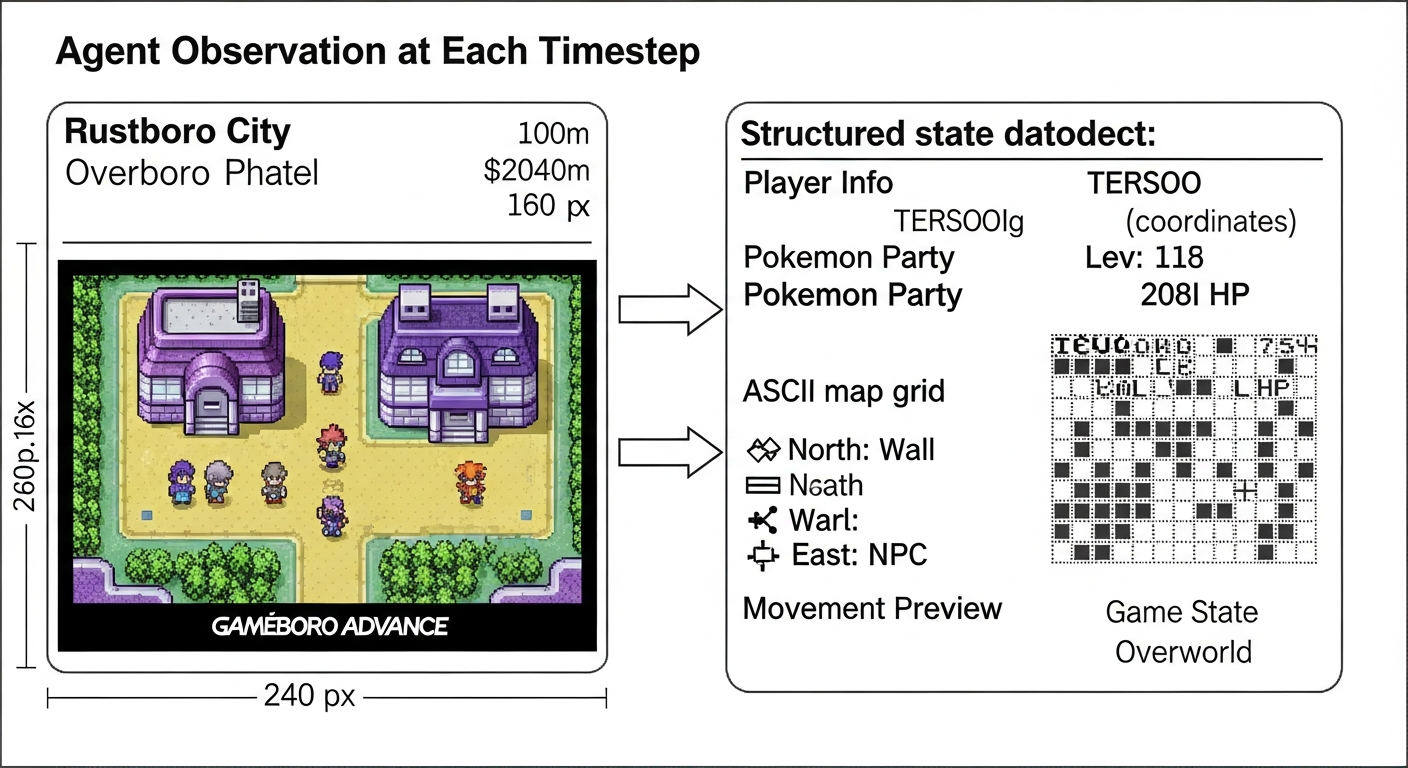
\includegraphics[width=\linewidth]{ch3/agent_perspective_draft.png}
\caption{\textbf{Agent Observation at Each Timestep.} At each step, the agent receives both a raw visual frame (left) and a structured text state (right) derived from memory extraction and pre-parsed map data. The vision-language model processes both modalities simultaneously to ground its reasoning and action selection. \tersoo{Refine this draft figure with actual screenshot and formatted text state.}}
\label{fig:agent_perspective}
\end{figure}

The VLM processes both modalities simultaneously. The visual frame grounds spatial awareness and captures information not available in the structured state and which would otherwise need substantial engineering effort to deduce. Menu navigation, for instance, is a crucial competency that the agent must successfuly demonstrate---the position of the cursor is provided entirely through visual cues \tersoo{note: add a figure here for reference of menu navigation in the bag}. Structured text provides precise numerical data and map topology that serve to increase observability. Our benchmark also supports a vision-only setting, though our experiments do not evaluate in this setting. This dual-modality design is a deliberate choice. We aim to provide enough structured state text information to effectively gauge the reasoning and action capabilities of frontier agents in a more natural domain while preserving visual reasoning as a necessary component for benchmark progress. Further details on state extraction and the role of porymap decompilation data appear in Appendix~\ref{sec:appendix_environment}.

\subsubsection{The World from Our Perspective}\label{sec:our_perspective}

Complementing the agent's observation interface is the evaluation interface designed for human observers. Inspired by the speedrunning community's emphasis on transparency and real-time verification, the interface provides a live view of four concurrent information streams: (1) the Pok\'{e}mon Emerald game screen showing the current game state, (2) agent reasoning traces appearing as logs detailing strategy and action rationale, (3) the current party composition (4) the agent's objectives, and (5) an ASCII map overview with button-action history (Figure~\ref{fig:ch3_eval_interface}).

\begin{figure}[t]
\centering
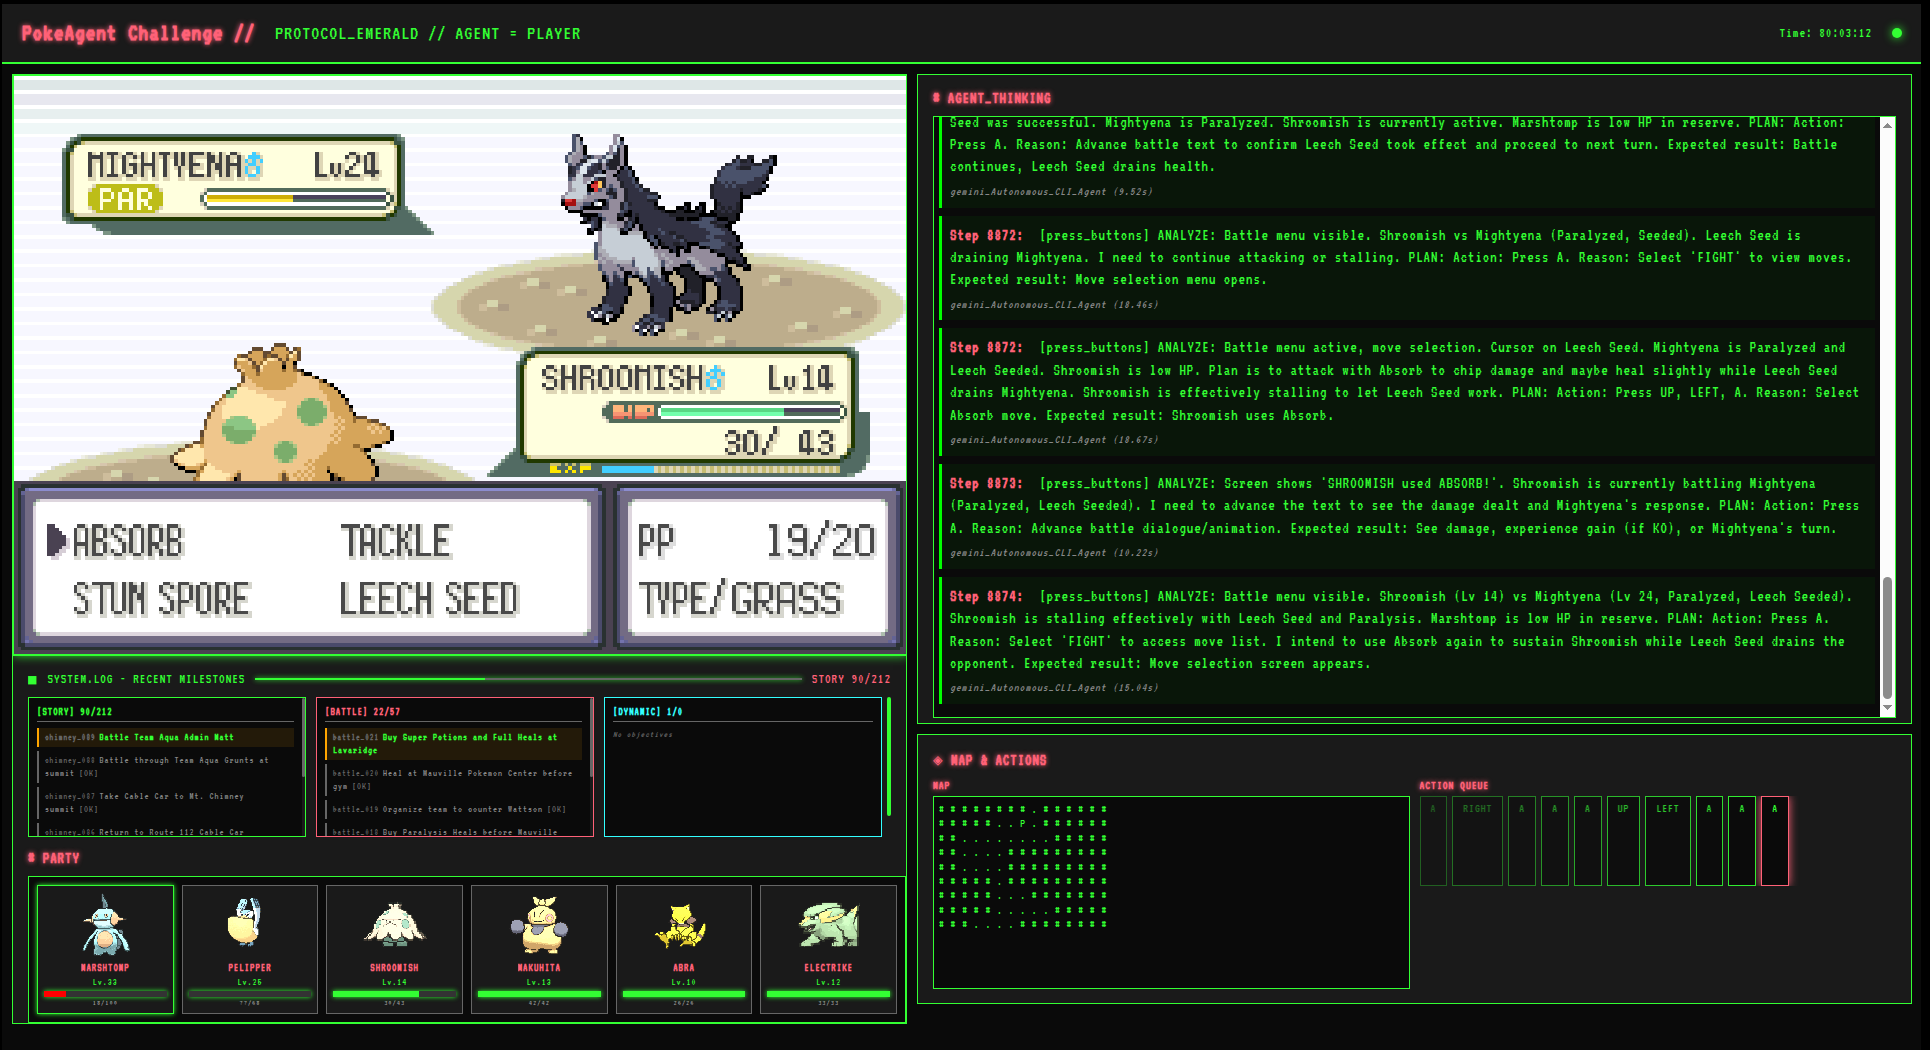
\includegraphics[width=\linewidth]{ch3/layout.png}
\caption{\textbf{Speedrunning Track Evaluation Interface.} The interface displays: (1) the game screen showing a trainer battle (top left), (2) agent reasoning traces with timestamped decision logs (right panel), (3) party composition with sprite previews (bottom left), (4)  objectives (bottom left), and (5) map overview with action history (bottom right). This visualization enables real-time observability into agent behavior.}
\label{fig:ch3_eval_interface}
\end{figure}

This interface enables real-time debugging across the thousands of timesteps that speedrunning requires. Evaluators can observe not only what the agent does but also the reasoning behind each action. This level of observability is essential for the qualitative analysis discussed in Section~\ref{sec:qualitative_analysis} and for identifying the failure modes that motivate the architectural decisions in Chapters~4 and~5.

\subsubsection{Tutorial}\label{sec:tutorial}

The tutorial setting evaluates agents on the opening segment of Pok\'{e}mon Emerald, spanning 15 milestones from the player's starting location in Littleroot Town through defeating the first gym leader, Roxanne, in Rustboro City. Milestone completion is inferred via the ROM. Figure~\ref{fig:ch3_speedrun_route} illustrates the route and its milestones.

\begin{figure}[t]
\centering
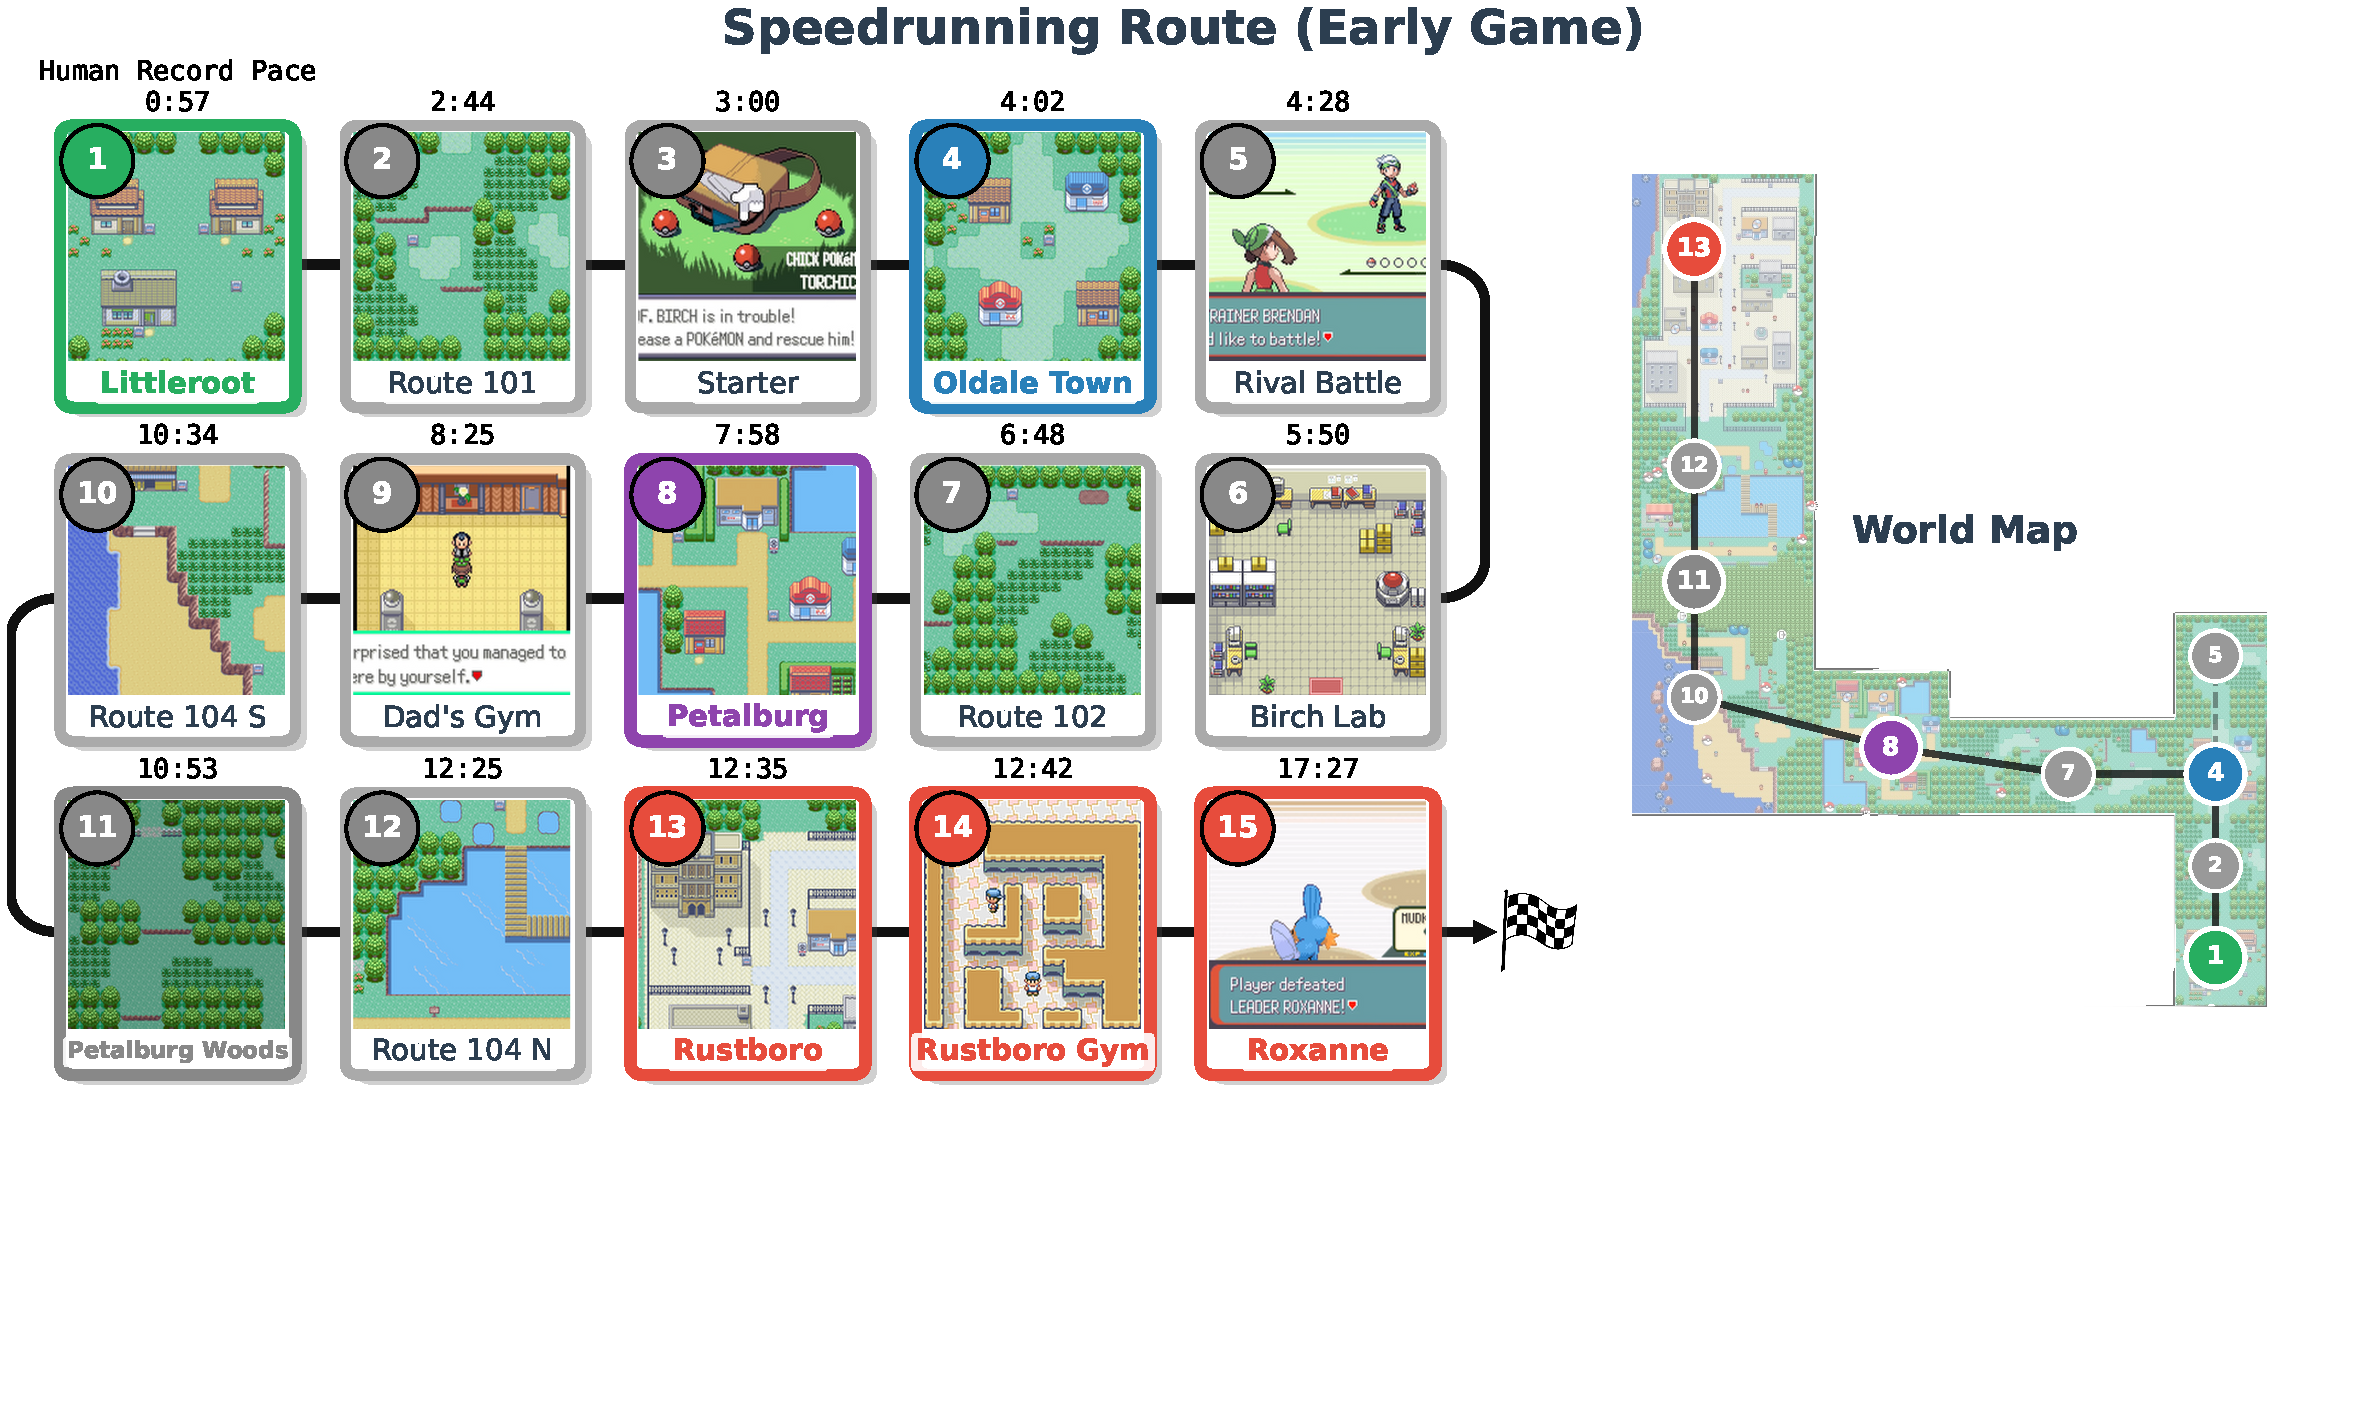
\includegraphics[width=\linewidth]{ch3/speedrun_route.pdf}
\vspace{-18mm}
\caption{\textbf{Speedrunning Route (Early Game).} Milestones from Littleroot Town (1) to Defeating Roxanne (15), with game frames from each waypoint. The geographic overview (right) maps key locations. Although progression appears linear, the route requires substantial exploration and backtracking---agents must revisit earlier areas, navigate branching paths, and manage nonlinear dependencies between objectives. \tersoo{Note: cite https://www.speedrun.com/pkmnemerald/runs/yvpvw74y as the world record speedrun}}
\vspace{-4mm}
\label{fig:ch3_speedrun_route}
\end{figure}

This segment serves as a minimal competency test: it exercises the full stack of capabilities an agent must possess---visual perception, dialog processing, menu management, overworld navigation, wild and trainer battles, and basic resource management---while remaining short enough to enable rapid iteration at reasonable cost. Top human speedrunners can complete this segment in as little as 18 minutes, while the average human player required approximately 80 minutes. The best frontier models complete this segment in under three hours.

The tutorial is the simplest setting that must pass reliably before testing in longer-horizon settings becomes valuable. An agent that cannot consistently navigate from Littleroot to Rustboro, manage its inventory, and defeat the first gym leader (Roxanne) has no prospect of reliably succeeding through the game's later, substantially more complex segments. By standardizing this segment as the first evaluation tier, we provide a controlled environment for isolating basic competency failures from the higher-order reasoning challenges that emerge in extended play. A detailed walkthrough of each milestone and the competencies it tests appears in Appendix~\ref{sec:appendix_tutorial_walkthrough}.

\subsubsection{Long Horizon}\label{sec:long_horizon}

The long-horizon setting extends the evaluation through the third gym leader, Wattson, in Mauville City. Experiments in this setting routinely exceed 12 hours of wall-clock time and require the agent to maintain coherent behavior across several thousands of reasoning steps. This extension transforms the benchmark from a focused competency test into a comprehensive evaluation of long-context autonomous behavior.

\begin{figure}[t]
\centering
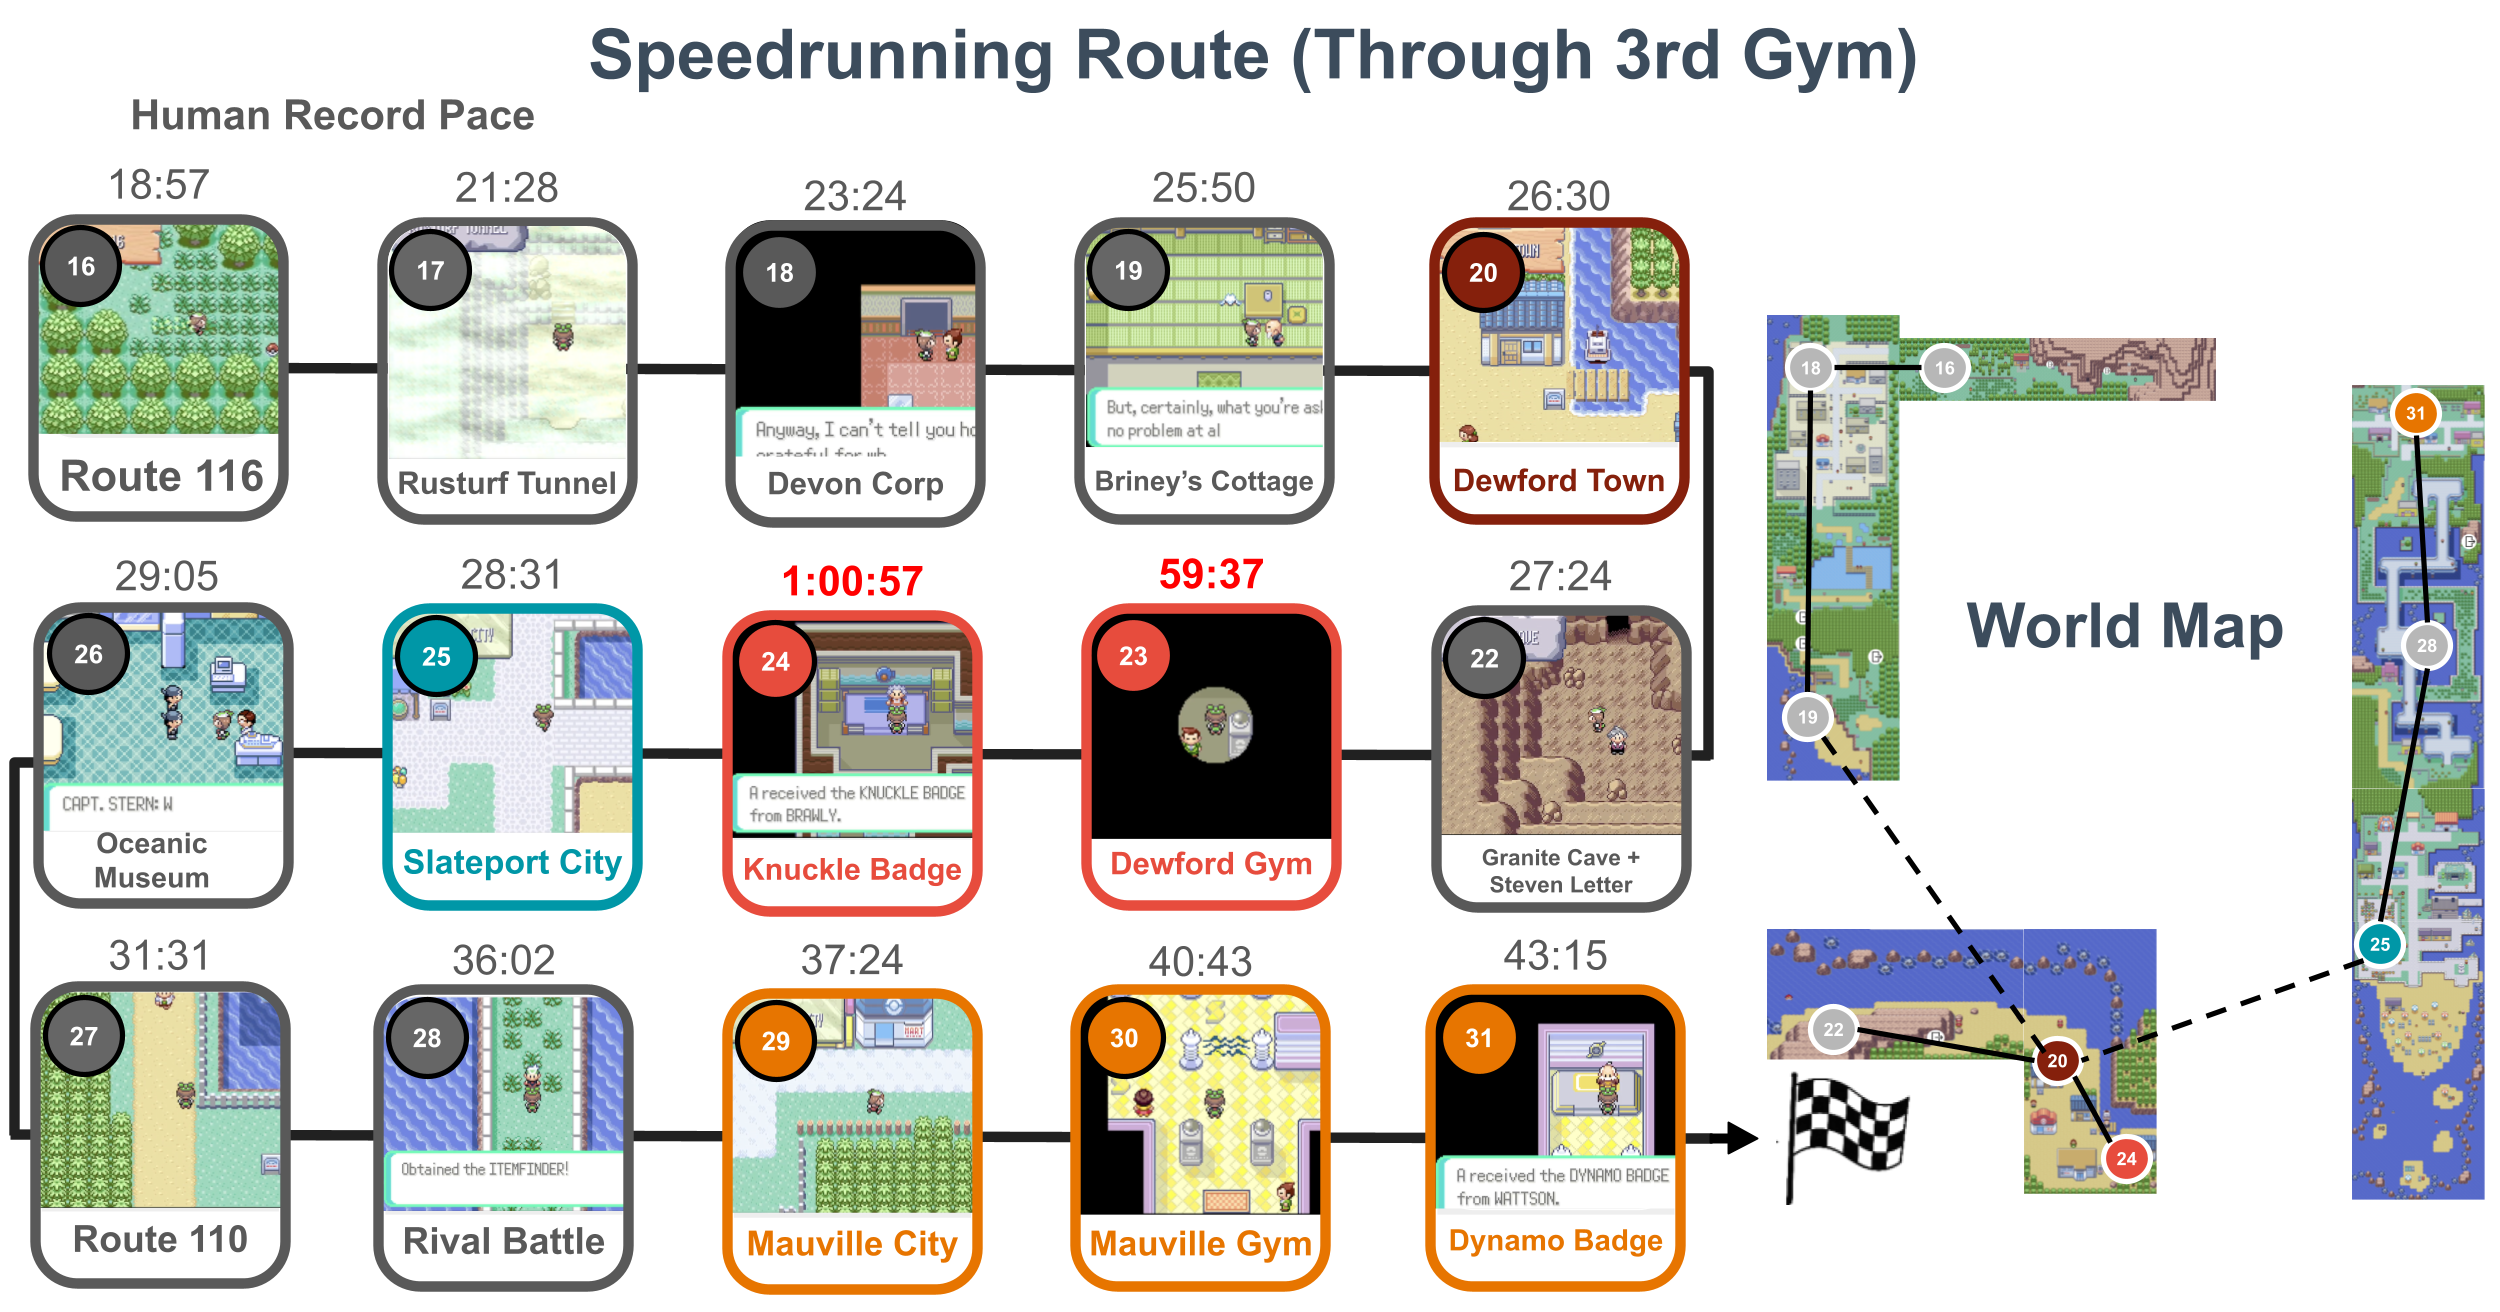
\includegraphics[width=\linewidth]{ch3/long_horizon_route.png}
\caption{\textbf{Long-Horizon Route (Through Gym 3).} Extended progression from Littleroot Town through Rustboro City (Gym 1: Roxanne), Dewford Town (Gym 2: Brawly), and Mauville City (Gym 3: Wattson) across a total of 16 additional objectives. After the first gym, progression becomes non-linear as interconnected storylines. The gym quest, Team Aqua encounters, and the Devon Corporation delivery create dependencies that constrain completion ordering. Note that Gym 2 and Gym 3 can be completed in any order; top human speedrunners complete Gym 3 before Gym 2 as it offers more efficient pathing.  \tersoo{NOTE: cite https://www.speedrun.com/pkmnemerald/runs/yvpvw74y as the world record mGBA speedrun}}
\label{fig:ch3_long_horizon_route}
\end{figure}

Beyond the first gym, the game's structure shifts qualitatively. Two features distinguish the long-horizon setting from the tutorial.

\paragraph{Increased non-linear progression.} After defeating Roxanne, the player must navigate interconnected storylines that block one another. The main gym quest (Roxanne $\to$ Brawly $\to$ Wattson) is interleaved with the Team Aqua/Magma narrative arc and key-item fetch quests (the Devon Corporation delivery to Steven in Granite Cave, Mr.\ Briney's ferry service). Completing one storyline often requires progress in another: the player cannot reach Dewford Town and obtain the second gym badge without first resolving the Rusturf Tunnel encounter with Team Aqua and earning Mr.\ Briney's assistance. These dependencies create a topological ordering structured around key event rather than a strict linear sequence. As the horzion over which evaluation takes place increases, the set of valid orderings expands substantially, and small routing decisions concering gym attempt order, whether to grind levels or push forward with the current state of the party, when to heal---have downstream consequences on speed, navigation time, and resource management.

\paragraph{Compounding complexity.} The agent's Pok\'{e}mon team grows and evolves, requiring increasingly sophisticated resource management: choosing which Pok\'{e}mon to catch and train, which moves to teach, when to heal, and how to allocate limited funds across Pok\'{e} Balls, Potions, and other consumables. Trainer battles grow more difficult, demanding type-awareness and strategic switching. Navigation distances increase, and without careful planning, frequent backtracking and rerouting becomes expensive. The agent must reason about its own cumulative progress by recalling which areas have been explored, which items collected, and which NPCs spoken to, across a session log that now stretches into many tens or hundreds millions of tokens. This is precisely the setting where long-context coherence, precise use of persistent memory structured planning abstractions become essential. A detailed walkthrough of the extended route appears in Appendix~\ref{sec:appendix_longhorz_walkthrough}.


\subsection{Speedrunning Evaluation Criteria}\label{sec:evaluation_criteria}

\begin{figure}[h]
\centering
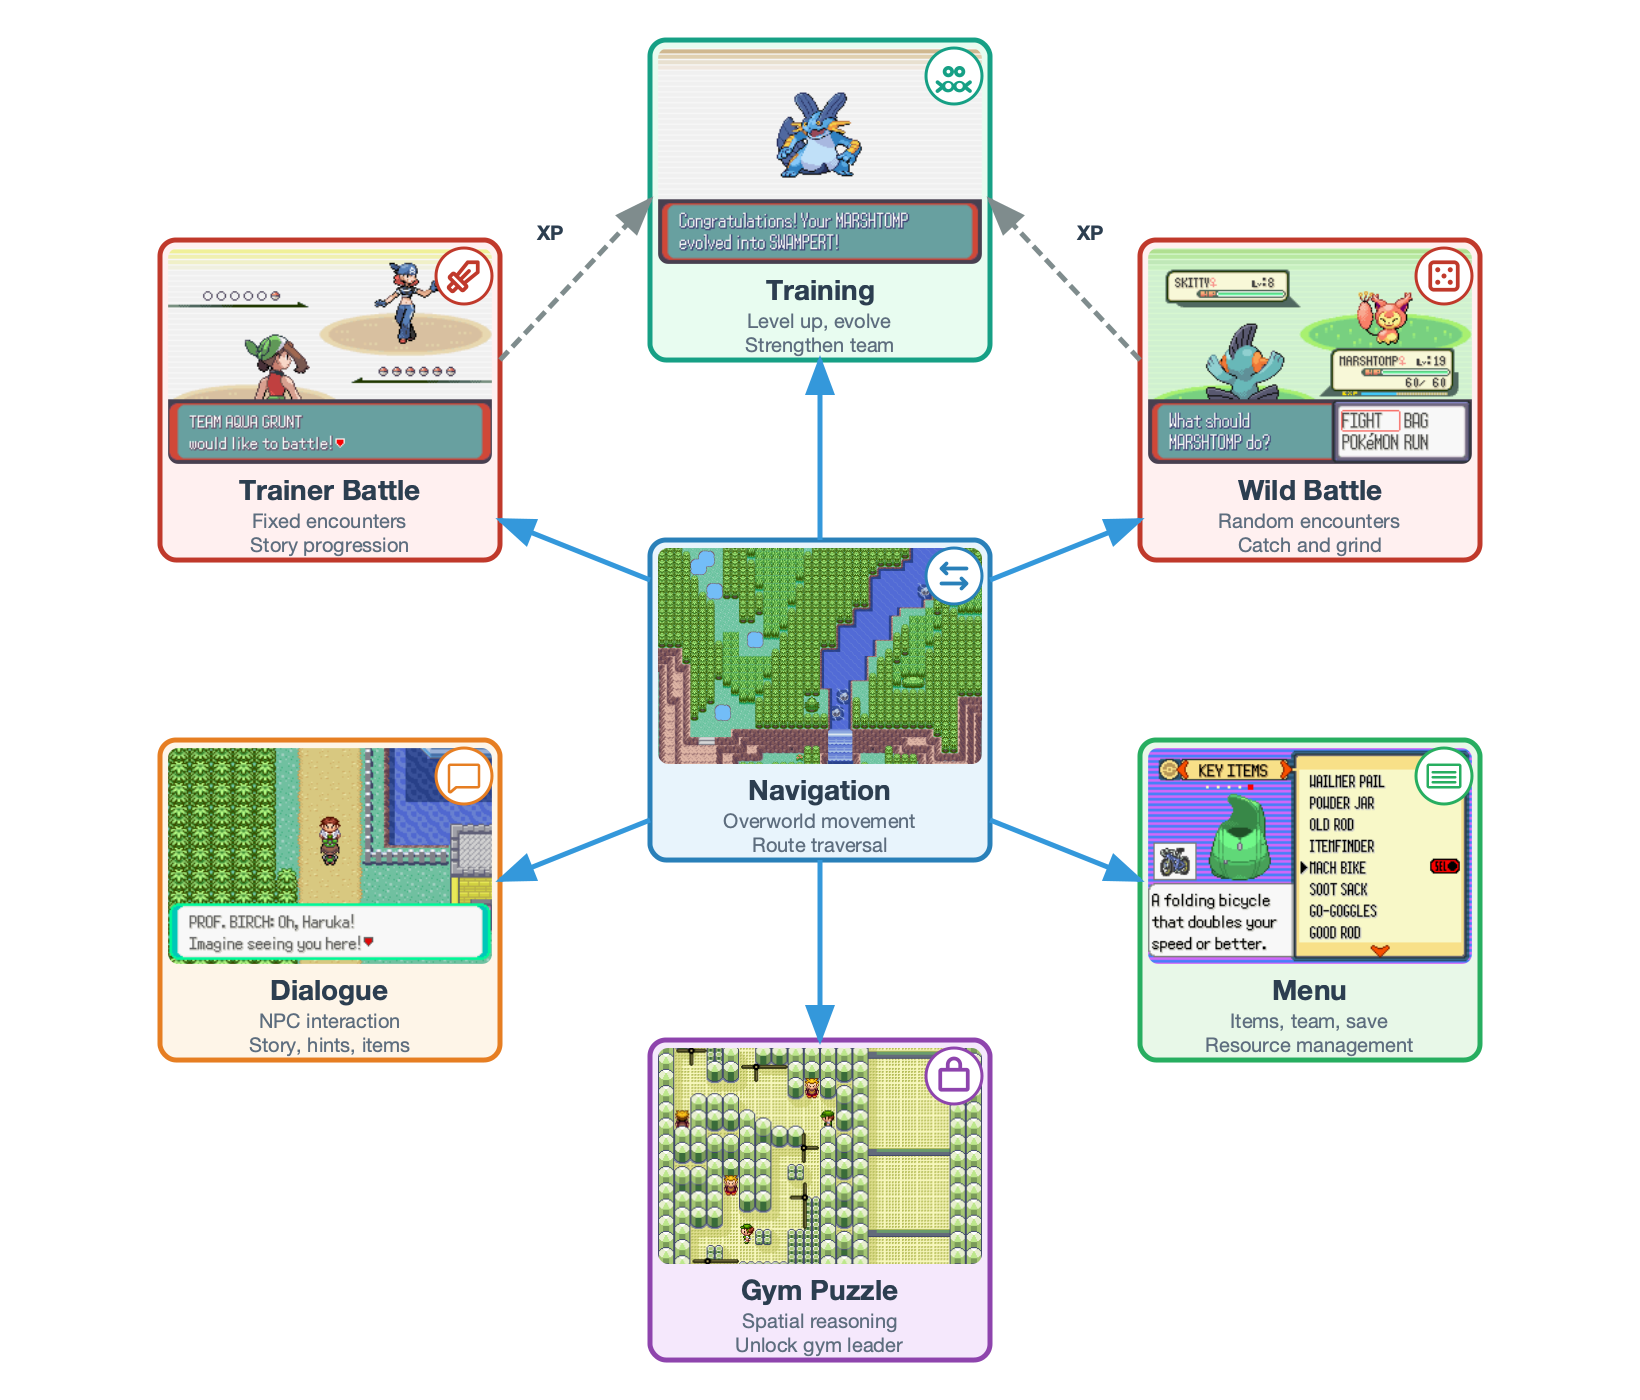
\includegraphics[width=\linewidth]{ch3/track2_tasks.png}
\caption{\textbf{Speedrunning Track Task Diversity.} Directed graph showing RPG subtask categories and their dependencies. Core tasks include overworld navigation, battle encounters (wild and trainer), gym puzzles, menu management, and NPC dialogue. Edges indicate how completing one task type enables or requires others---for example, navigation leads to encounters, battles yield experience for team building, and menu interactions manage resources needed for all other tasks.}
\label{fig:ch3_task_diversity}
\end{figure}

Evaluating agent performance in an extremely open-ended RPG requires metrics that capture both efficiency and behavioral quality. We measure performance along two complementary axes: quantitative metrics that provide objective, directly comparable results, and qualitative analysis that capture a richer set of behavioral nuances that numbers alone simply cannot convey. Figure~\ref{fig:ch3_task_diversity} illustrates the diverse and interconnected subtasks that agents must navigate, motivating why a single metric is insufficient.

Infrastructure details concerning the cumulative metric logging system, agent reasoning trace collection, and tool-call recording are described in detail in Appendix~\ref{sec:appendix_infrastructure}.

\subsubsection{Quantitative Metrics}\label{sec:quantitative_metrics}

We define four primary quantitative metrics, encompassing the most relevant axes of agent performance.

\paragraph{Completion Percentage.} The most fundamental metric is milestone completion: the fraction of standardized checkpoints an agent reaches before the experiment terminates. Milestones are captured implicitly as the agent progresses through the game, providing a dependent variable that reflects cumulative capability. In the tutorial setting, this ranges from 0 (failing to leave the starting house) to 100\% (defeating Roxanne). In the long-horizon setting, milestones extend through the third gym. Completion percentage provides a coarse but robust metric of agent performance.

\paragraph{Wall-Clock Time.} Among agents that achieve comporable completion results, wall-clock time serves as an important ranking metric. Unlike most game AI benchmarks that pause the emulator between actions \tersoo{cite!}, our environment runs continuously in real time reflecting the dynamic setting in which real agent systems operate. This makes wall-clock time a joint measure of decision quality and computational throughput. We nonetheless recognize that internal benchmark infrastructure related to---among other things---metric collection, client-server communication, and data persistence as well as the hardware any given experiment runs on confound this measurement. In spite of this, more efficient pipelines involving models that better balance low latency with reasoning acumen will generally perform better along this axis relative to other models.

\paragraph{Cumulative Actions.} We define an \emph{action} as a completed request-response pair from the foundation model over which a given harness is constructed. Each action may involve multiple tool calls within a single step, and depending on the tool used and the game state, may trigger a multitude of button-actions. Cumulative action count measures sample efficiency: how many deliberation cycles the agent requires to reach a given milestone. Models that strike a balance between chaining together multiple tool calls within a single step while respecting real-time environment dynamics---the frames and time required to interact with items, NPCs, and location transitions---will score better on this metric. Action count is particularly informative when contrasted with wall-clock time: Deepest completed the NeurIPS competition route in just 649 actions (the fewest of any team) despite ranking 5th by time, revealing a tradeoff between inference speed and action efficiency. \tersoo{note: since i moved the results for the benchmark, its important to now reference these results wherever they appear}

\paragraph{Cumulative Tokens and Cost.} We track a global view of token consumption across reasoning and tool calls, as well as the corresponding API cost. This metric captures the economic dimension of agent deployment: harnesses with effective caching strategies can consume more tokens at a lower cost, while reasoning-heavy models tend to be substantially more expensive per step. The cost metric also reflects the interaction between model choice and harness design---a harness that minimizes redundant context by compacting trajectory windows and caching repeated observations will incur lower costs even when using a more expensive frontier model.

\subsubsection{Qualitative Analysis}\label{sec:qualitative_analysis}

Quantitative metrics provide objective rankings but may obfuscate the behavioral mechanisms that drive performance differences. Our qualitative analysis examines agent behavior across both success and failure modes, recognizing that the various aspects of agent capability are deeply interconnected in their effect on overall performance.

Take, for example, the tradeoff between model capability and harness exploitation. A weaker model may exhibit lower per-turn latency, but if it lacks the capacity for effective tool use and fails to consistently store memories, ground its actions in visual perception, or effectively plan, then its downstream performance will will suffer. Such agents frequently enter loops, repeatedly attempting the same failed action while their reasoning traces reveal confusion about why progress has stalled. Conversely, a more powerful model may be slower on a per-turn basis, but if it effectively leverages the harness's memory, planning, and perception tools, its actions tend to be less confused, leading to steadier progress and fewer CRF cases.

\paragraph{Success Modes.} We descrige effective agent behavior along several dimensions: the ability to use planning abstractions for both near-term actions and longer-term route optimization; effective memory management that maintains awareness of prior progress, collected items, and explored areas; accurate visual perception that enables reliable localization and map-based reasoning; and creative problem-solving when encountering novel situations such as gym puzzles or unexpected obstacles. Successful agents often exhibit interesting emergent behaviors visible in their reasoning traces. For instance, reasoning about type advantages before a gym battle affecting the party composition, or deciding to improve the level of its party via explicit training objectives prior to attempting to defeat a gym leader so as to avoid slowing down its progress in the event of failure. 

\paragraph{Failure Modes.} Failure manifests along the same dimensions. The observe that the most common and consequential failure mode, across a variety of harness designs and model families is poor visual perception: when the agent misidentifies what is shown on the game screen, misreads on-screen text, or fails to ground its reasoning in what it observes in the visual frame, the resulting errors in localization and mapping cascade through planning and action selection. A second class of failure involves inadequate use of memory and planning abstraction. Agents that fail to record or retrieve information about completed segments of the game suffer in their ability to localize their progress within the structure \pokemon{} Emerald narrative, leading to downstream degradation in objective planning. Behaviorally, this tends to manifest in re-visitation of irrelevant locations or reattempting completed segments of the game. A third, more abstract failure mode is derivative of the aforementioned failure modes. \textbf{Catastrophic Reasoning Failure (CRF),} \tersoo{NOTE: make sure that I'm using CRF here-on out} is the state in which a compounding sequence of errors leads the agent into a virtually unrecoverable state. In the best case, while greatly slowing progress and ballooning computational costs, these states are still recoverable; in the worst case, the dissonance between what the agents belief over the set of valid actions and what the current game state actually requires for progress will irreconcilably derail a run. These qualitative observations are best obtained through live analysis of agent reasoning alongside the emulated game instance, but can also be conducted at larger scale through LLM-based approaches of processing of the agent logs and metric data that our benchmark infrastructure records.

% ---------------------------------------------------------------------------
\subsection{Speedrunning Baselines}\label{sec:baselines}
\tersoo{NOTE: edit this section for better flow}
Before analyzing the evolution of the \pokeagent{} harness in the ensuing chapter, we establish the a top human-speedrun by player, \textit{keepingiticy}, on the widely accepted speedrunning platform, speedrun.com \tersoo{NOTE: properly cite - https://www.speedrun.com/pkmnemerald/runs/yvpvw74y}.

\subsubsection{Human Baselines}\label{sec:human_baselines}

Top human speedrunners provide the absolute performance ceiling for agent comparison across both the tutorial and long-horizon settings. The top human speedrunner who goes by the name \textit{keepingiticy}, completed the tutorial setting in 17 minutes and 27 seconds and the long-horizon setting (through the aquisition of 3 gym badges) in 1 hour and 57 seconds, representing the upper bound on what is achievable with perfect game knowledge and precise motor execution. At the other end, the average non-speedrunning human player may require, by our estimation, 1.5 hours to complete the tutorial setting and anywhere from 4 to 8 hours to complete the long-horizon setting. 

% ============================================================================
% Chapter 4: PokeAgent Baseline Harness
% ============================================================================

\newpage
\section{PokeAgent Baseline Harness}\label{sec:pokeagent}

This chapter traces the development of the \pokeagent{} harness from its simplest form during the \pokeagent{} Challenge NeurIPS 2025 competition through to the realized expert system we deploy as a performance ceiling in the ensuing AutoEvolve experiments in Chapter~\ref{sec:autoevolve}. The narrative follows a chronological arc across three distinct phases of development: (1)~the \emph{competition era} harness--- aptly referred to as \textbf{\pokeagent{} Simplest}---in which a minimal four-module agent participated in the NeurIPS 2025 challenge; (2)~in transitioning from competition to an \emph{open benchmark} we built upon learnings from the simple agent to an intermediate harness which introduced structured objectives, a knowledge base, and A* pathfinding to produce the baseline results reported in the \pokeagent{} Challenge Retrospective~\citep{karten2025pokeagent}; and (3)~the \emph{expert harness} $\mathcal{H}_{\text{expert}}$, a fully realised multi-agent orchestration system engineered for state-of-the-art performance in the long-horizon setting and which provides the human-crafted ceiling against which AutoEvolve is measured in Chapter~\ref{sec:autoevolve}.


% ---------------------------------------------------------------------------
\subsection{Early Development: \pokeagent{} Simple Era}\label{sec:early_development}

The earliest \pokeagent{} harness, deployed as a baseline for the NeurIPS 2025 competition, was a minimal system built to validate whether frontier VLMs could make meaningful progress in Pok\'{e}mon Emerald at all. This system received visual frames and structured state text in accordance with our environment design though it employed no external tools as the agent could only output raw GBA button presses; a rolling short-term buffer of its action history was its only memory abstraction. Finally, it followed an explicitly constructed observe-plan-act loop embedded within its four-module design.

\subsubsection{Four-Module Pipeline}\label{sec:four_module}

\pokeagent{} Simplest implemented a linear pipeline of four modules, three of which backed by a separate VLM call:

\begin{enumerate}[nosep]
    \item \textbf{Perception}: receives the $240 \times 160$ game frame and structured state text; produces a textual scene analysis classifying the current context (overworld, battle, dialog, menu) and a flag indicating whether the situation requires deliberate reasoning.
    \item \textbf{Planning}: receives the memory context and current plan from the previous agent; checks whether the existing plan has been accomplished and, if so, generates an updated plan covering immediate goals, short-term objectives, and long-term strategy.
    \item \textbf{Memory}: involves no external calls to an LLM; maintained purely as a rolling buffer of 50 entries of observation--action pairs. \texttt{deque}. It programatically extracts significant events (map transitions, battle entries/exits) and formats the recent history into a context string, in accordance with pre-defined textual-parsing heuristics.
    \item \textbf{Action}: receives all accumulated context (memory, plan, perception, visual frame, state text) and produces a list of up to 10 Game Boy Advance (GBA) button presses (\texttt{A}, \texttt{B}, \texttt{UP}, \texttt{DOWN}, \texttt{LEFT}, \texttt{RIGHT}, \texttt{START}, \texttt{SELECT}).
\end{enumerate}

Each step through this pipeline required 3 VLM calls, making the agent slow on a per-action basis. Importantly, it introduced a rudimentary objective system at the point of the planning module as it prompted the agent to maintain dynamic objectives that it could create or complete via inline commands (\texttt{ADD\_OBJECTIVE:}, \texttt{COMPLETE\_OBJECTIVE:}). The system prompt was minimal by design with just two sentences describing the agent's role, and no access to MCP tools, long-term memory abstractions in the form of a knowledge base, and no mechanism for self-reflection. The agent navigated purely by interpreting the ASCII map, relying on the foundation model's world knowledge and spatial reasoning to infer appropriate movement. Despite these limitations, it was sufficient to complete the tutorial setting, establishing a proof of concept that frontier VLMs could play Pok\'{e}mon Emerald with minimal scaffolding.


\begin{figure}[t]
\centering
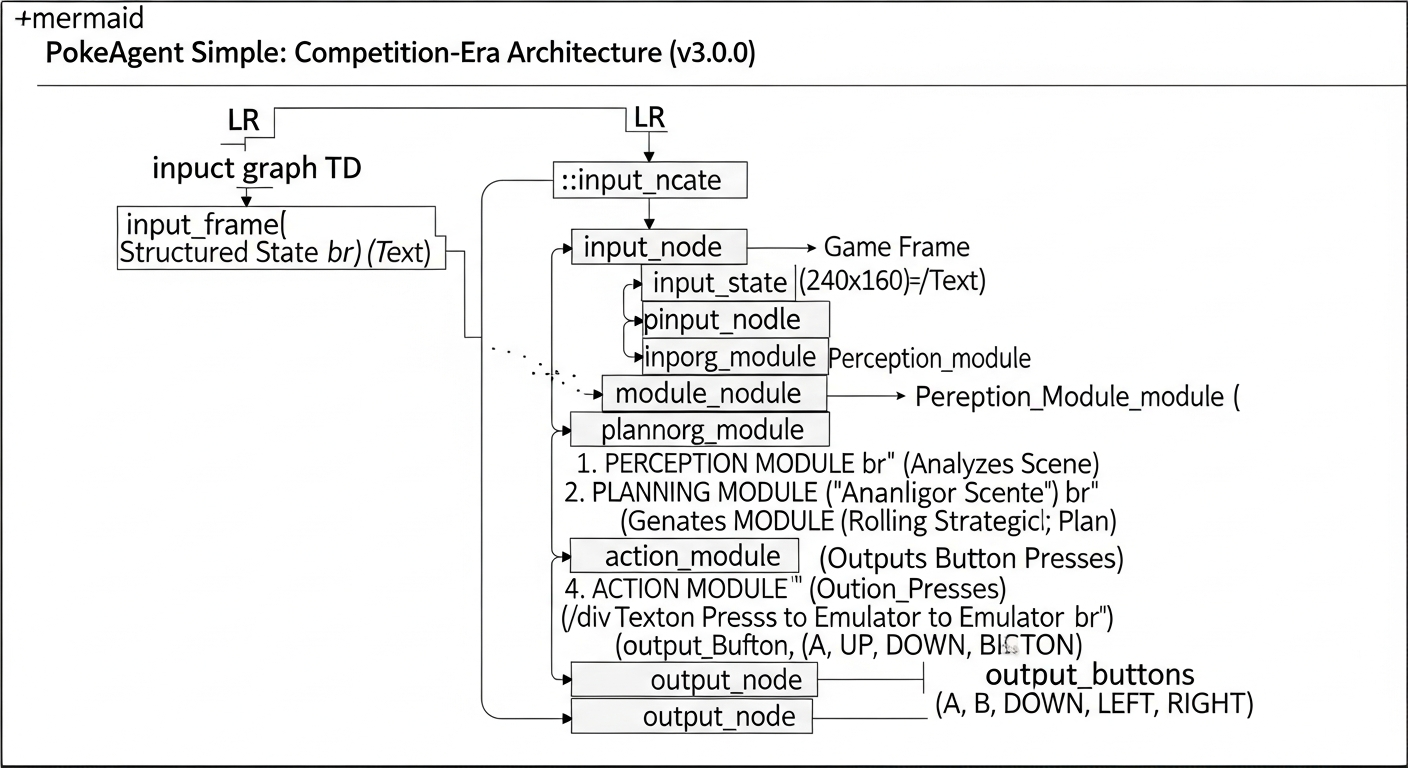
\includegraphics[width=0.85\linewidth]{ch4/simple_agent_draft.png}
\caption{\textbf{PokeAgent Simple: Competition-Era Architecture.} The four-module pipeline (Perception $\to$ Planning $\to$ Memory $\to$ Action) processes a game frame and structured state through sequential VLM calls, producing button presses. The SimpleAgent variant collapses this into a single structured VLM call. Neither variant has access to external tools or persistent memory.}

\tersoo{TODO: Refine this draft figure with a cleaner diagram.}
\label{fig:ch4_simple_agent}
\end{figure}

% ---------------------------------------------------------------------------
\subsection{Early Performance}\label{sec:early_performance}

A fundamental limitation of the four-module pipeline was its perception bottleneck. The Perception module translated a raw $240 \times 160$ game frame into a textual scene description, and all downstream modules (Planning, Memory, Action) operated exclusively on this text. The Action module never saw the original image. This architecture is analogous to a human who must act on an environment they cannot see, relying entirely on a second person's verbal description of the scene---a description that is inevitably lossy, filtered through that person's judgment about what information is relevant. In our setting, the Perception module would routinely omit tile-level details (e.g., ledge positions, NPC facing directions) that proved critical for navigation, while over-emphasizing salient but less actionable features such as the names of visible Pok\'{e}mon species. The result was an information bottleneck that constrained action quality regardless of the Action module's reasoning capability. Later iterations of the harness addressed this by providing the visual frame directly to the action-generating VLM call, eliminating the intermediate textual translation.

\subsubsection{NeurIPS 2025 Competition Results}\label{sec:competition_results}
\begin{figure}[h]
\centering
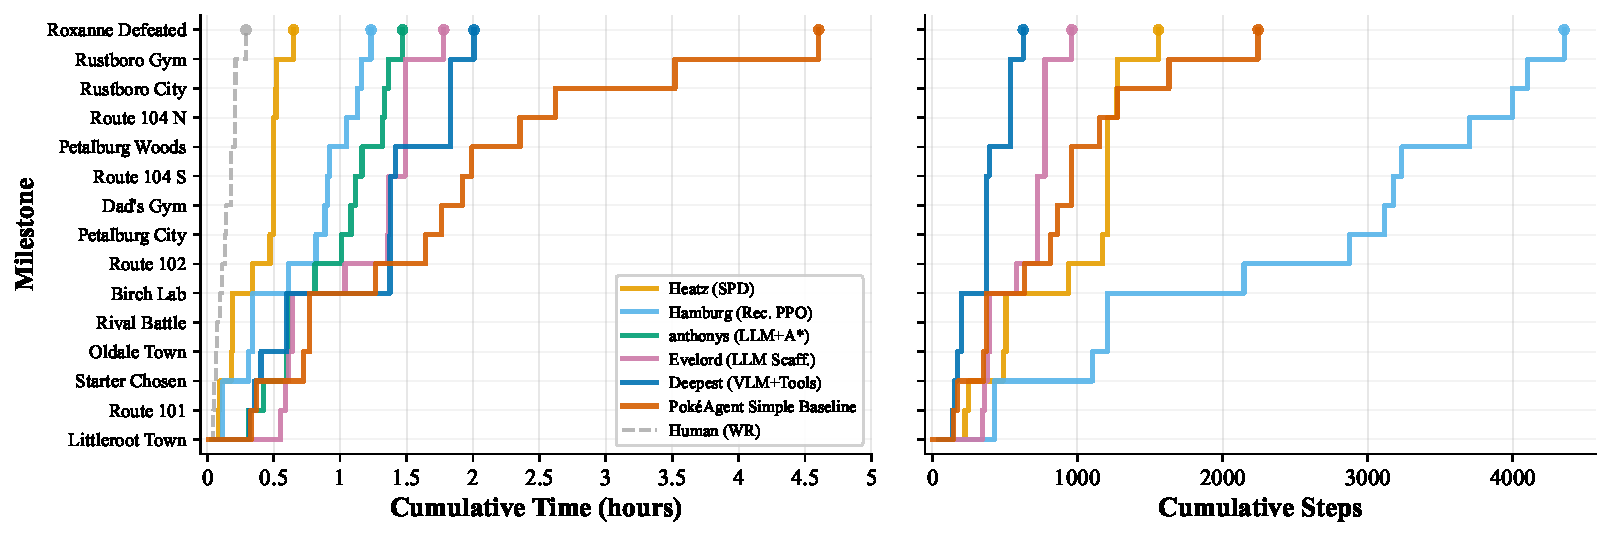
\includegraphics[width=\linewidth]{ch3/track2_progress_time.pdf}
\caption{\textbf{NeurIPS Speedrunning Leaderboard.} Milestone progress vs.\ wall-clock time (left) and cumulative agent steps (right) for the six teams that completed all 15 milestones. Team Deepest (Judge's Choice) completed in the fewest steps (649) despite ranking 5th by time, highlighting the tradeoff between inference speed and action efficiency. \pokeagent{} Simplest was both time and step-poor.}
\label{fig:ch4_neurips_leaderboard}
\end{figure}

The NeurIPS speedrunning competition (Figure~\ref{fig:ch4_neurips_leaderboard}) produced six teams that achieved 100\% milestone completion, with completion times ranging from 40:13 (Heatz) to 2:46:48. The diversity of approaches is instructive. At the top, Heatz's Scripted Policy Distillation (SPD) method leveraged an LLM to decompose the task into subgoals with executable success conditions, generate scripted policies for each, and distill these into neural networks refined via RL---achieving emergent behaviors including BFS-based local pathfinding and trainer battle skipping~\citep{karten2025pokeagent}. Hamburg Pok\'{e}Runners took second with a pure RL approach: recurrent PPO with a CNN-MLP encoder, LSTM for temporal reasoning, and a binary milestone vector that served as both memory and goal conditioning. Anthonys (third place) combined deterministic A* pathfinding with phase-based prompt templates, decomposing the game into seven distinct phases with specialized navigation strategies. Deepest received the Judge's Choice award for sample efficiency, completing the route in just 649 actions (fewest of any team) using a training-free architecture built around a guidebook system, image-based goal recognition, and adaptive reasoning budgets. Full methodology descriptions for each team are provided in Appendix~\ref{sec:appendix_competitor_methods}.


A key insight from the speedrunning competition is the consistency that specialist methods display in outperforming generalist LLM approaches in the tutorial setting. The winning team, Heatz, completed the route in 40:13---nearly twice as fast as the second-place Hamburg Pok\'{e}Runners, who also employed RL-based approach. The remaining completions all used LLM harness architectures with varying levels of tool integration. Nevertheless, LLMs played a central role in the winning approach: the LLM provided the prior (task structure and initial behavior) while RL provided refinement (faster execution and strategy discovery). This pattern of using LLMs for high-level reasoning and RL for low-level optimization suggests a fruitful direction for future work; we discuss the scalability of LLM--RL hybrid approaches in Section~\ref{sec:future_work}.

The PokeAgent Simple baseline, by contrast was the weakest of the LLM harness approaches. Several observations from its performance spurred subsequent development. First, the release of Gemini 3 models led to a notable increase in performance, particularly around visual processing. Actions appeared more visually grounded, with less overreliance on text state~\citep{google2025gemini3}. Tasks requiring precision tile-level movement, orientation, and interaction, such as setting the clock in the player's bedroom, became much more consistent. This confirmed that base model capability, especially in its ability to natively reason across multiple input modalities, was a first-order driver of performance. Second, the four-module architecture was poor on both step and time efficiency, requiring 3 VLM calls per action, prompting us to increase the efficiency of our action-generation pipeline. Third, the agent lacked coherence across extended play: it would frequently become confused about game progress and infer its next action solely from the current screen and its world knowledge, making slow but eventual progress through the tutorial's largely linear structure. A common failure mode followed the completion of the rival battle in Route 103 (see Figure ~\ref{fig:ch3_speedrun_route} for reference). Upon returning back to Oldale Town, the agent would often attempt to proceed westward to Route 102 without first traveling further south to visit Professor Birch in Little Root Town. Decreasing the prevalence of this failure mode would necessitate a more powerful abstraction for planning.



\subsubsection{Intermediate Harness Improvements}\label{sec:benchmark_results}

Following the competition, the \pokeagent{} harness underwent its first major revision, introducing several architectural changes that substantially improved consistency and speed in the tutorial setting:

\paragraph{Objective System.} The most impactful addition was an explicit objective system that separated planning from action execution. Rather than relying on the underlying model to implicitly maintain a sense of progress through a combination of its world knowledge and action history, the new harness explicitly maintained a sequence of objectives that could be generated dynamically by the agent or pre-defined from a walkthrough source~\citep{bulbapedia2025walkthrough}. To support this new system for planning, we additionally exposed research tools to the agent for obtaining progress and walkthrough summaries. By isolating planning into a distinct phase, the agent could develop structured plans and execute them systematically, reducing the frequency of CRF modes. At this stage, the objective system was an append-only log whose successful employment required accurate completion detection. In the absence of tools enabling replanning, the premature marking of, or failure to denote critical objectives as completed could still lead to unrecoverable states.

\paragraph{Knowledge Base.} A persistent knowledge base abstraction allowed the agent to store discoveries (locations visited, items found, NPCs locations, storyline insights) in a flat list with importance-weighted retrieval. This gave the agent a mechanism for localizing its progress within the game narrative when generating new plans, improving consistency in execution.

\paragraph{A* Pathfinding.} Our initial observations of \pokeagent{} Simple's elucidated the difficulty that even frontier VLMs have in successfully traversing EAEs. Recent evaluations confirm that LLMs struggle with coordinate-based navigation and spatial reasoning tasks, with performance degrading sharply as environment complexity increases~\citep{yamada2024evaluating}, and that agentic LLMs and VLMs exhibit particularly poor navigation performance in game environments~\citep{paglieri2024balrog}.  The integration of A* pathfinding abstracted away most of reasoning burden into a programtic tool. The agent could now request navigation to specific coordinates or warp points, with the pathfinder computing optimal routes and introducing optional randomness that respected tile traversability, collision boundaries, and ledges. This reduced navigation failures dramatically, though the addition of a programmatic tool with such a strong coupling to game state decreased the generality of the harness by imposing an additional engineering burden. Reducing this dependence on hand-crafted pathfinding---for example, through learned spatial representations or SLAM-like map construction---is a direction we discuss in Section~\ref{sec:future_work}.


\subsubsection{Open Benchmark Results}\label{sec:open_benchmark_results}

\begin{figure}[h]
\centering
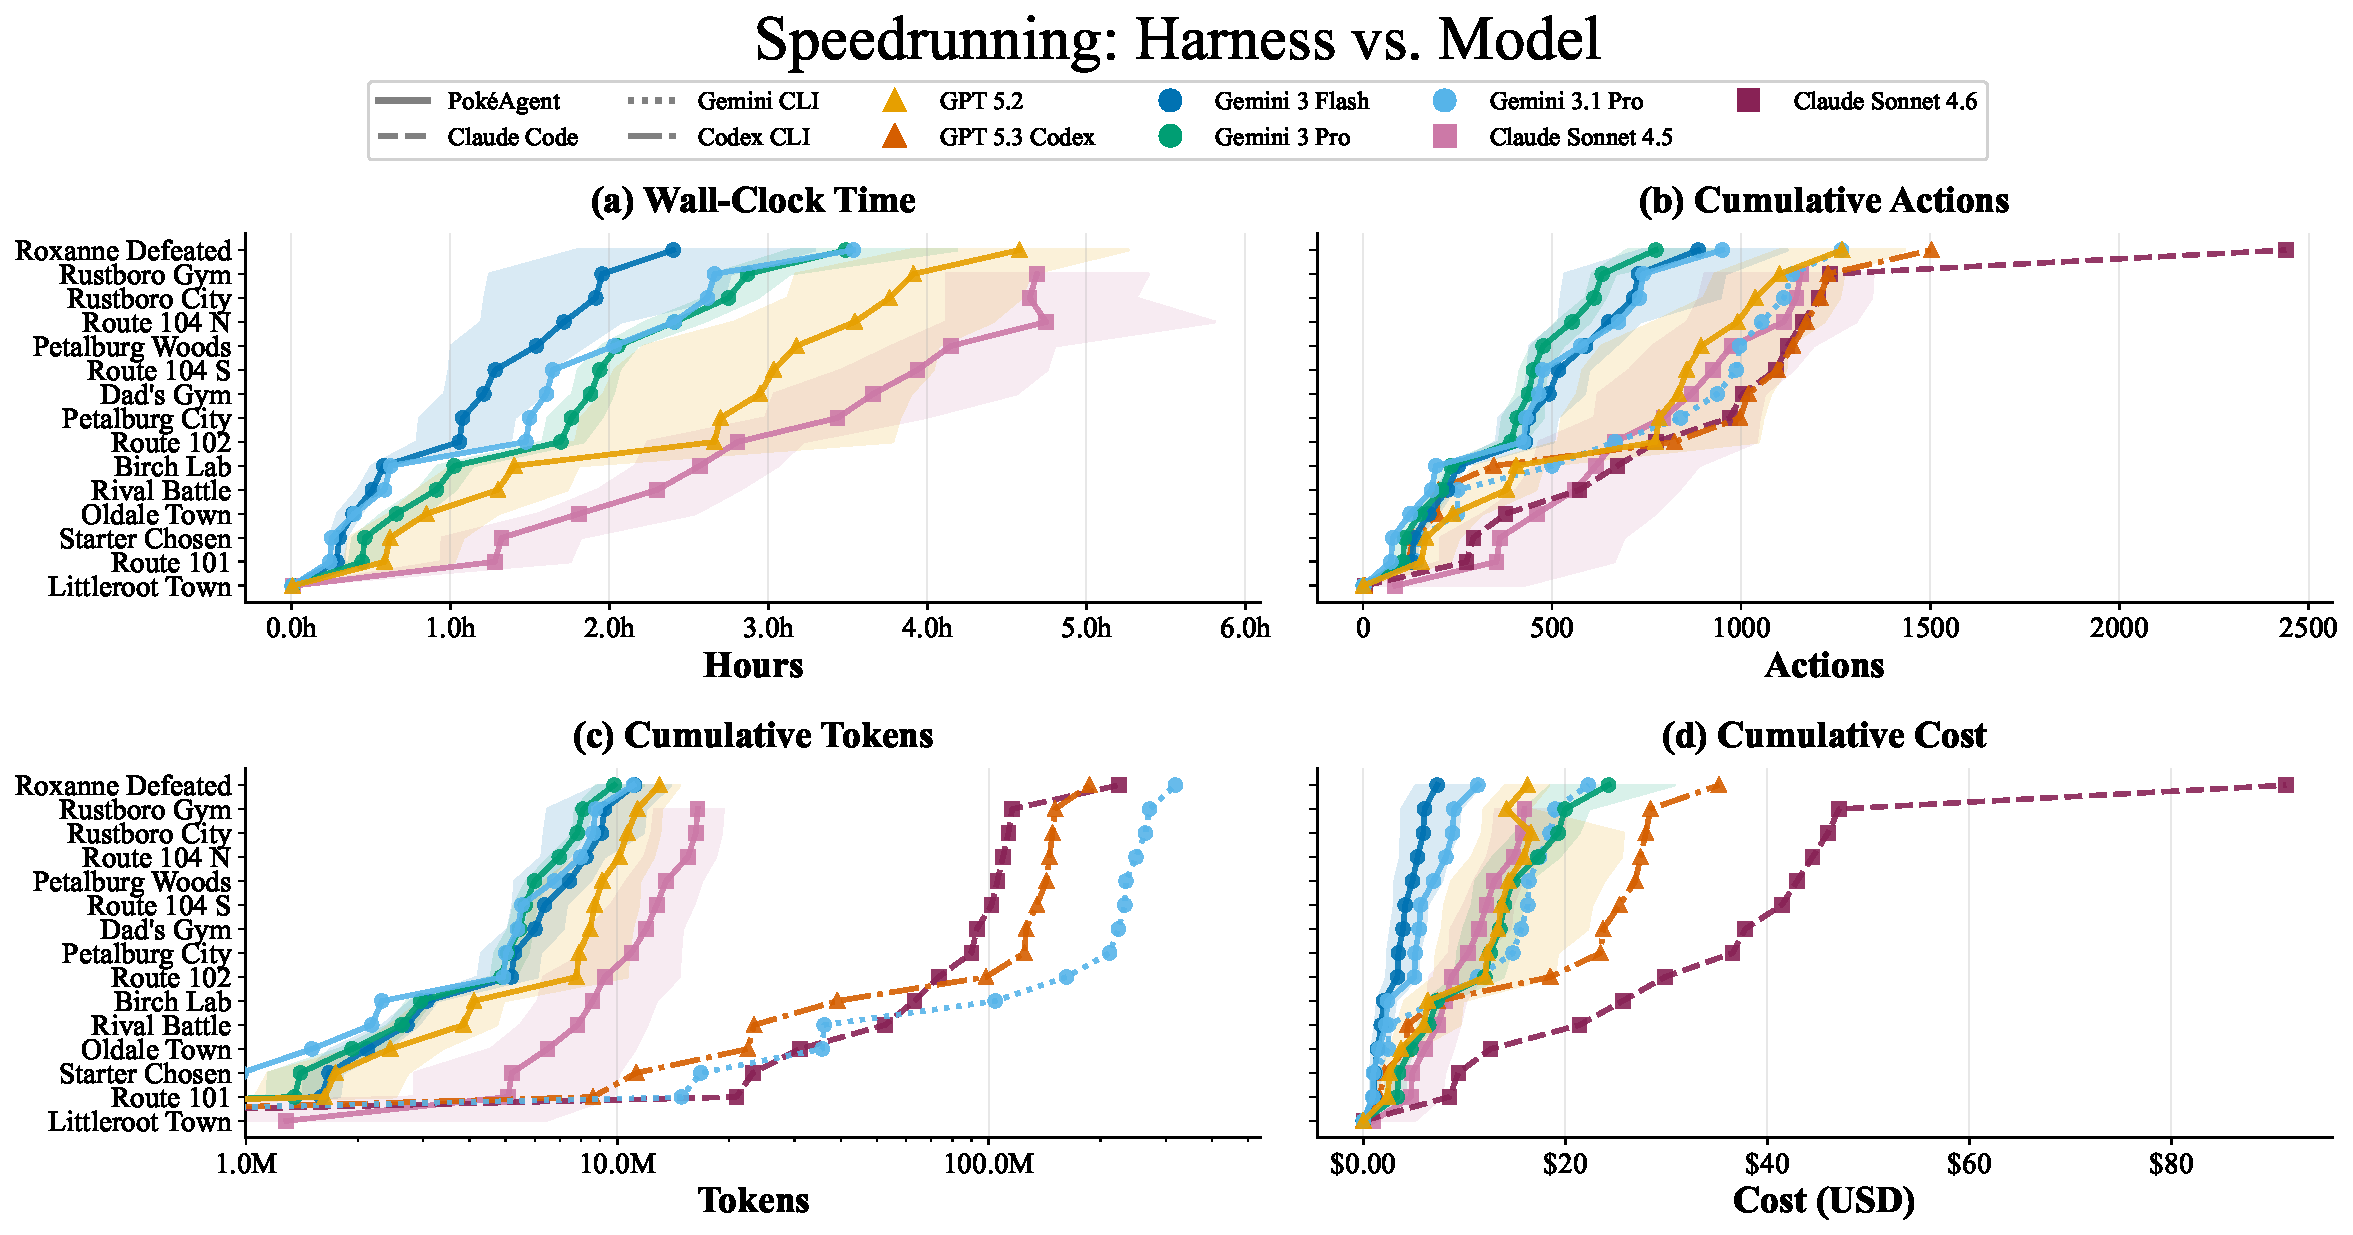
\includegraphics[width=\linewidth]{ch4/milestone_confidence.pdf}
\caption{\textbf{Speedrunning Harness vs.\ Model Comparisons (Tutorial Setting).} Cumulative wall-clock time, actions, tokens, and cost at each milestone for five frontier models on the \pokeagent{} harness (mean $\pm$ min/max range across runs). Gemini 3 Flash completes the route fastest ($\sim$2:24 mean) but requires more actions than Gemini 3 Pro. Claude Sonnet 4.5 completes all milestones but with the highest variance and 3--4$\times$ the cost of Gemini variants. GPT-5.2 falls between the two families.}
\label{fig:ch4_harness_vs_model}
\end{figure}


\paragraph{Model Comparisons.} A consistent finding across models is that Gemini outperforms in visual reasoning, despite Claude and GPT models being generally regarded as stronger on text-only benchmarks~\citep{chiang2024chatbot, google2025gemini3}. Gemini models exhibited more reliable visual grounding: they would almost always select Mudkip as their starter, with reasoning traces explicitly noting its type advantage against the Rock-type first gym. Claude and GPT models were less consistent in this regard, affecting downstream battle performance and completion speed for the tutorial segment. While not directly relevant to our harness-level analysis---which does not involve training or weight updates---this observation nonetheless suggests that domain-specific world knowledge is a meaningful differentiator for performance even among frontier models.

\paragraph{Harness Comparisons.} The retrospective also evaluated three proprietary CLI agents harnesses: Claude Code, Codex CLI, and Gemini CLI. We provided these harnesses with access to three MCP tools for retrieving game state, pressing buttons, and pathfinding. These coding-focused agents bring powerful native abstractions: context windows on the order of 200,000+ tokens before compaction, strong Pok\'{e}mon world knowledge, and proprietary problem-solving scaffolding that enables hypothesis exploration and online research. Several qualitative observations stood out. Their native planning systems, while effective for software engineering tasks, operated at a level of granularity that was often insufficiently specific for RPG navigation---plans like ``go to Rustboro City'' lack the operational detail needed for reliable execution. Their proprietary scaffolding allowed them to explore hypotheses directly in the embodied setting and use online research tools to redirect when stuck, but at the cost of significantly higher token burn. These results underscored that while powerful general-purpose harnesses can make meaningful progress out of the box---especially when equipped with external tools like pathfinding---the non-linear, long-horizon exploration characteristic of RPG play benefits from domain-tailored abstractions. We return to this observation in Section~\ref{sec:future_work}.

% ---------------------------------------------------------------------------
\subsection{Towards an Expert Harness}\label{sec:towards_subagents}

The results and subsequent improvements made to our harness over the prior two implementations made clear a set of architectural gaps in the harness that could not be addressed by incremental improvements. Two external trends reinforced the direction of development.

\paragraph{Model Capability Improvements.} The transition from Gemini 2.5 to Gemini 3 models brought substantial improvements in multimodal reasoning~\citep{google2025gemini3}. Actions became more visually grounded, with the agent demonstrating finer control over movement and more reliable interpretation of in-game text and navigation of menus. Tasks that had been prohibitively difficult for Gemini 2.5, such as accurately setting the bedroom clock or reading small menu text, became reliable with the Gemini 3 family of models. We likewise observed improvements to the consistency of tool-calling via decreases in the incidences of  passing invalid arguments or erroneously formatted parameters. For instance, Gemini 2.5 models would sometimes call \texttt{PRESS-BUTTONS['QUICK ATTACK']} or \texttt{PRESS-BUTTONS['CLOCK']} rather than using \texttt{PRESS-BUTTONS['A']} when attempting to select a move or interact with a particular item. This progress suggested that a more capable VLM would improve both the agent's intrinsic reasoning and its reliability in using the harness's tool interface.


\paragraph{Subagent Orchestration.} In parallel, the rapid maturation of agent frameworks in the software engineering domain through the likes of Claude Code, Cursor, Codex CLI, and Gemini CLI, demonstrated the power of subagent architectures for managing context in long-horizon tasks~\citep{cursor2026scalingagents}. These systems introduced planning tools, persistent memory, and eventually subagent delegation as first-class primitives. Their success in coding tasks provided a compelling template for embodied agent design, as demonstrated by their out-of-the-box generalization to our speedrunning benchmark. The advent of subagent orchestration, a paradigm wherein a primary orchestrator agent delegates atomized tasks for subagents (equipped with their own context window) to complete, was of particular interest due to its effectiveness in preventing \textit{context rot}\footnote{Context rot refers to the progressive degradation of an agent's reasoning coherence as its context window accumulates irrelevant or contradictory information over many turns. This phenomenon is documented in the context of recursive language models~\citep{zhang2025rlm} and observed directly in long-horizon Pok\'{e}mon play~\citep{gemini2p5report}.}. As we observe, the loss in coherence as a result of context rot is a relevant failure mode within the \pokemon{} Emerald setting where the agent may forget subtle details as it attempts to complete a difficult task over many turns or when switching between overworld, battle, or menu states. Improving the handling of battles was a notable area of improvement as a common failure mode involved the agent mistaking a trainer battle for a wild encounter and wasting resources attempting to catch another trainer's \pokemon{}.

\paragraph{Self-critique.} Emerging work on self-adaptive agent systems demonstrated the value of self-critique abstractions~\citep{madaan2023selfrefine, shinn2023reflexion}. Without such mechanisms, agents cannot meaningfully adjust their policy when stuck, increasing the probability that a failure mode cascades into CRF and requiring manual intervention via system prompt edits (the full prompt is reproduced in Appendix~\ref{sec:appendix_prompts}). This manual approach does not scale to long-horizon experimentation where it is unreasonable to analyze the agent's reasoning traces over multiple hours of execution.

Two recurring failure modes illustrate the need for self-critique. First, the agent was sensitive to the naming and granularity of objectives: an objective like ``route\_104\_south'' would cause the agent to navigate to the southernmost tile of Route~104 rather than recognizing the label as a distinct map section preceding Petalburg Woods. Without a mechanism to detect and correct this misinterpretation, the error would cascade into downstream objective failures. Second, maps with many warp points overwhelmed the agent's ability to select the correct destination, producing loops of navigation to incorrect warps that the agent could not self-diagnose. Both failure modes share a common structure: the agent lacks the ability to step back, evaluate whether its current approach is working, and adjust. As demonstrated by Self-Refine~\citep{madaan2023selfrefine} and Reflexion~\citep{shinn2023reflexion}, equipping agents with mechanisms for verbal self-evaluation can break these failure loops before they become irrecoverable.

These observations motivated the refactoring of the intermediate harness design along several specific abstractions as we looked to improve performance in long-horizon settings. Our expert harness ($\mathcal{H}_{\text{expert}}$) supports (1) subagent delegation for improved context management and defines several custom subagents along with general subagent primitives for orchestrating agent to define at runtime, restructures the Knowledge Base and action-history into (2) persistent hierarchical short and long term memory, introduces (3) a skill library, (4) sandboxed code execution to allow the agent to prototype and deploy their own custom tools, and (5) refactors the objective system to enable the dynamic replanning.

% ---------------------------------------------------------------------------
\subsection{System Design: Expert Harness}\label{sec:system_design}

The expert harness $\mathcal{H}_{\text{expert}}$ is a multi-agent orchestration system and represents a distinct qualitative departure from its preceding architectures: rather than a monolithic observe-plan-act loop, $\mathcal{H}_{\text{expert}}$ decomposes the agent into a central orchestrator that is equipped with a subset ($\mathcal{T_O}$) of the available tools including tools for creating and calling subagents, set of specialized subagents ($\mathcal{S_O}$), persistent stores (subagents, skills, memories), and a sandboxed execution environment. This system is engineered specifically for the long-horizon setting described in Section~\ref{sec:long_horizon}. As we will see, it accepts a modest penalty in per-step efficiency because of the overhead introduced by frequent context switching between orchestrator and subagents, in exchange for more stable performance and reduced incidences of CRF modes, over extended play across longer horizons.

We also formalize three scaffold configurations, at varying levels of sophistication, relevant to the ensuing chapter: \texttt{"\pokeagent{}"} ($\mathcal{H}_{\text{expert}}$) provides the full tool suite including built-in subagents, A* pathfinding, walkthrough access, and wiki lookup; \texttt{"Simple"} ($\mathcal{H}_{\min}$) strips away all built-in subagents, navigation tools, and research tools, leaving only raw button presses and the persistent stores; \texttt{"AutoEvolve"} ($\mathcal{H}_{\text{auto}}$) extends $\mathcal{H}_{\min}$ with a \texttt{HarnessEvolver} that mutates skills, subagents, and system prompts over time. The latter two configurations are central to the experimental design in Chapter~\ref{sec:autoevolve}.

\begin{figure}[t]
\centering
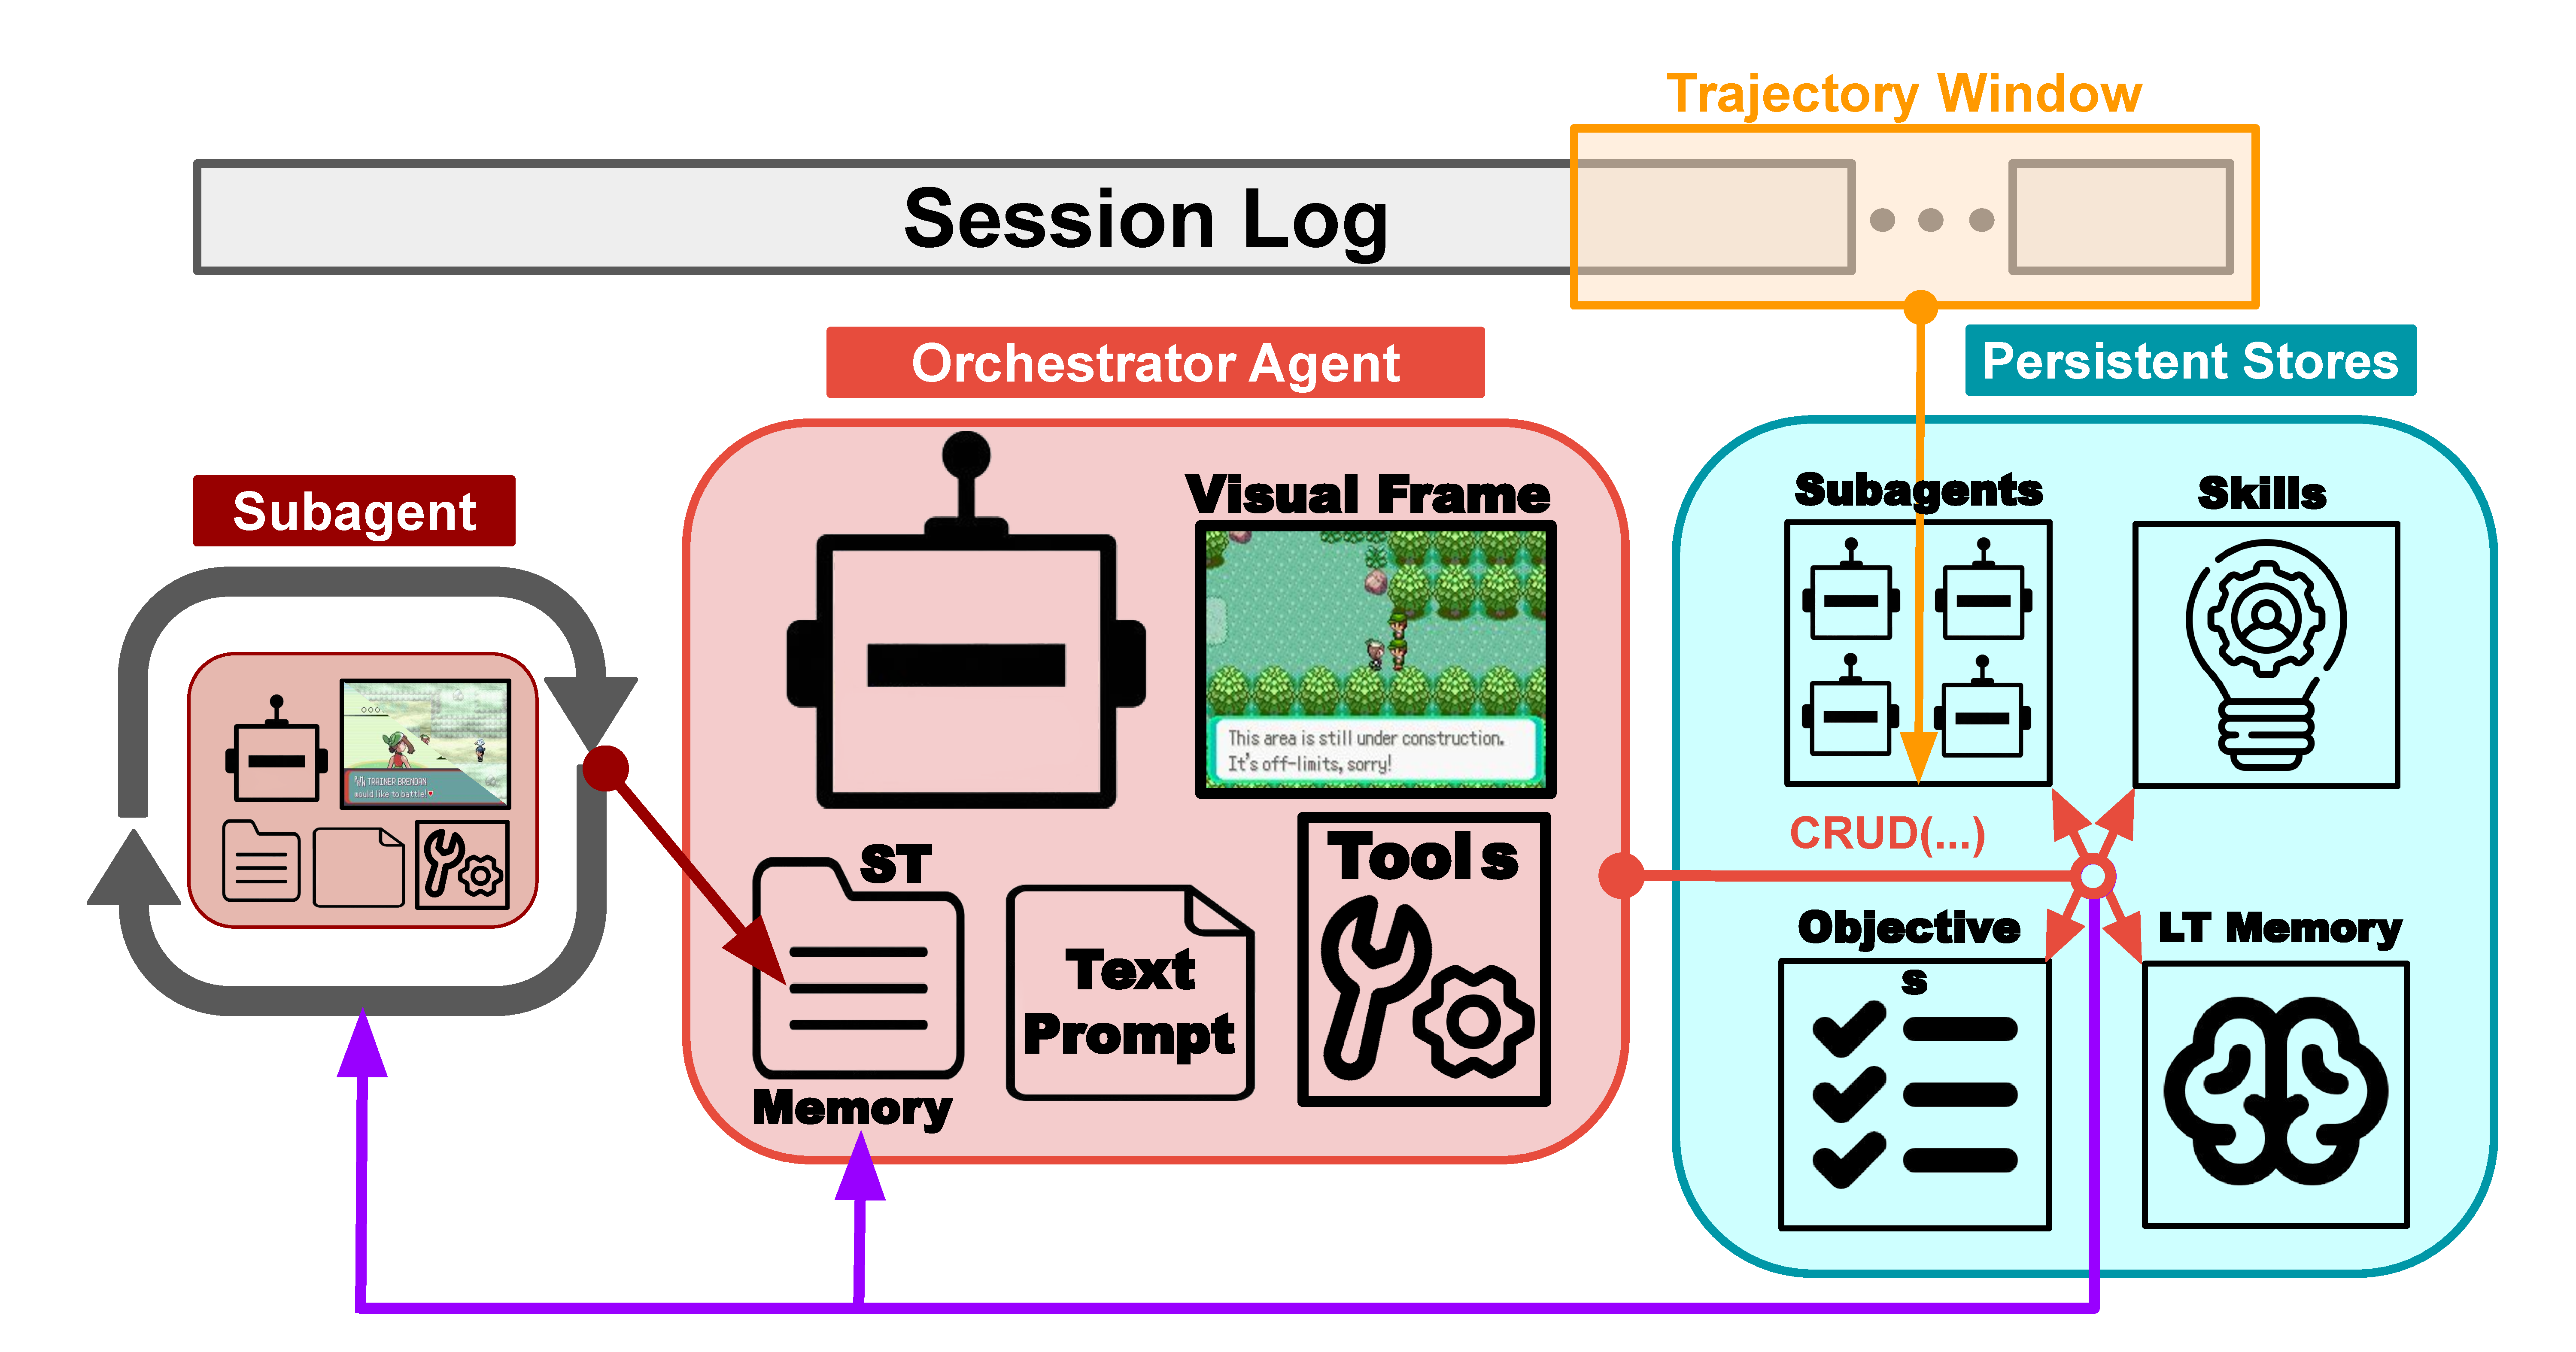
\includegraphics[width=\linewidth]{ch4/pokeagent_architecture.pdf}
\caption{\textbf{$\mathcal{H}_{\text{expert}}$ Multi-Agent Architecture.} The orchestrator coordinates subagents and MCP tools to play the game. Data flows left-to-right from the GBA emulator (game frames, parsed state) through the orchestrator (context management, subagent dispatch, stuck detection), which invokes either MCP tools (pathfinding, button inputs, knowledge retrieval) for direct game control or specialized subagents (battler, reflection, verification, gym puzzle, planner) for complex reasoning. A feedback loop returns compacted subagent outputs and tool results to inform subsequent decisions.}

\tersoo{TODO: Refine this draft with the full expert harness details (trajectory window, memory/skill/subagent stores, sandbox).}
\label{fig:ch4_expert_architecture}
\end{figure}

\subsubsection{Architecture Overview}\label{sec:architecture_overview}

At each step, the orchestrator fetches the current game state, assembles a structured prompt incorporating the short-term memory window, persistent store overviews, current objectives, and the visual frame, then queries the VLM and executes any resulting tool calls (Figure~\ref{fig:ch4_expert_architecture}). Every step must conclude with either a \texttt{press\_buttons} or \texttt{navigate\_to} call, preventing the model from deliberating indefinitely without advancing the game. When the orchestrator delegates to a subagent (e.g., the battler or planner), control transfers to a dedicated handler that runs its own multi-turn loop with a restricted tool set and fresh game state each turn. Upon termination, only a compacted summary returns to the orchestrator's short-term memory---not every inner turn. This context isolation prevents the orchestrator's context window from accumulating hundreds of battle or planning turns, enabling it to maintain coherence over thousands of high-level decisions. The following subsections detail each abstraction; a complete tool reference is provided in Appendix~\ref{sec:appendix_tools}.

\subsubsection{Trajectory Window}\label{sec:trajectory_window}

The trajectory window is a persistent global session log that records every agent step as a structured entry containing both the meta data associated with an agent step (step number, action taken, reasoning trace, outcome, location, and player coordinates) as well as full prompt passed to the VLM at that step---including the constituent structured text state. While it is also possible to include the image frame at these steps, the trajectory window that we employ does not save this information. This log takes inspiration from the treatmeant of global context by the RLM paradigm~\citep{qu2024recursive}. Rather than viewing the agent's history history as a flat, append-only context sequence, the trajectory is a structured, programmatically accessible workspace that the orchestrator process with the aid of subagents to query, analyze, and summarize any segment of execution history. We expose a tool (\texttt{process\_trajectory\_history}; see Table~\ref{tab:tool_defs} in Appendix~\ref{sec:appendix_tool_defs}) that allows the orchestrator to run ad-hoc analysis over arbitrary step ranges, enabling the agent to reason about patterns in its own behavior (e.g, verifying progress, reflecting on performance to unblock itself, etc).

% [Content moved to Chapter 5 -- trajectory window as bridge to AutoEvolve]


\subsubsection{Memory}\label{sec:memory}

The memory system implements a dual-layer architecture loosely inspired by the distinction between working memory and long-term memory drawn in cognitive neuroscience ~\citep{baddeley2000episodic, tulving1972episodic}. Reading from the short-term buffer---akin to human working memory--- is fast and automatic, while querying the long-term store requires an explicit tool call at higher latency in a way that mirrors the effortful retrieval from long-term memory. 

\paragraph{Short-term memory.} Both the orchestrator and any looping subagent internally maintain a buffer of the previous 20 tool calls---their parameters, success, and embedded agent reasoning. This buffer, formatted and injected into every prompt as the \textsc{Short-Term Memory} section, provides immediate context about recent actions and their outcomes. Additionally, compact overviews, organized as file-trees, of all three persistent stores (memory, skills, subagents) are injected every step, giving the orchestrator a birds-eye view of its accumulated knowledge without consuming excessive context.

\paragraph{Long-term memory.} The persistent memory store contrasts short-term memory by virtue of its tradeoff between increased latency for a virtually unbounded amount of data storage. This store supports CRUD operations with hierarchical path organization. Each \texttt{MemoryEntry} contains an identifier, a hierarchical path (e.g., \texttt{pokemon/team}, \texttt{events/gym\_battles}), a title, free-text content, the location and coordinates where it was created, importance (1--5), and tags. The tree overview renders entries as an indented hierarchy with \texttt{[id] title} leaves, providing a compact index that the VLM can scan to decide which entries to read into its short-term memory, update, add, or delete. Once a long-term memory is encoded within the short term memory as a tool-call result, it propagates there for a number of turns proportional the size of the short-term memory buffer. This asymmetry incentivizes the agent to maintain a compact, well-organized representation of its global knowledge, enabling the efficient retrieval of detailed knowledge.

\subsubsection{Skills}\label{sec:skills}

The global skill library extends the same process of storage and retrieval to behavioral and executable strategies that are learned at runtime and accessible to both the orchestrator and any subagents. Each skill contains a name, description, hierarchical path, empirical effectiveness rating (low/medium/high), and optionally a field containing executable Python code. The tree overview annotates executable code skills with \texttt{(run with: run\_skill)}, signaling to the VLM that these skills can be invoked directly.

Behavioral skills are textual: they encode strategies (e.g., ``when facing Rock-type gym leaders, lead with a Water or Grass type and use super-effective moves'') that an agent may optionally consult during reasoning. Executable skills contain Python code that runs in the sandbox (Section~\ref{sec:sandbox}) with access to game tools, enabling the agent to automate repetitive patterns---such as a training its team, navigation, or item acquistion---without replanning from scratch.

Agents manages skills in a similar fashion to memories as our harness exposes \texttt{process\_skill} (CRUD) and \texttt{run\_skill} (execution). 

% [Content moved to Chapter 5 -- skill library population in H_expert vs H_auto]

\subsubsection{Subagents}\label{sec:subagents}

The subagent system represents the most substial architectural divergence from prior iterations of our agent harness. It distinguishes between two types of subagents: \emph{1-step} subagents that perform a single VLM pass over the trajectory window without tool access, and \emph{delegated-loop} subagents that are callable from the orchestrator and run as autonomous multi-turn loops with their own restricted tool sets.

\paragraph{Built-in 1-step subagents.} $\mathcal{H}_{\text{expert}}$ exposes four pre-configured 1-step subagents that operate on the trajectory window and provide structured guidance (prompt text in Appendix~\ref{sec:appendix_prompts}):
\begin{itemize}[nosep]
    \item \texttt{reflect}: an external critique agent prompted to diagnoses stuck or looping states by analyzing the trajectory, returning an assessment with specific recommendations for strategy changes.
    \item \texttt{verify}: independently checks whether the current objective is truly complete, returning structured evidence for and against completion with a confidence score. This external oversight helps prevent the orchestrator from prematurely advancing when the agent incorrectly believes a task is finished.
    \item \texttt{summarize}: produces an unbiased trajectory summary, used for context compaction during context switches between the orchestrator and predefined subagents to preserve essential information while discarding redundant detail. Agents can optionally call this summarization tool ad-hoc.
    \item \texttt{gym\_puzzle}: provides domain-specific guidance for solving gym puzzles (e.g., Mauville's electric barriers) combined with current-state analysis.
\end{itemize}

\paragraph{Built-in delegated-loop subagents.} Two subagents run autonomous multi-turn loops:
\begin{itemize}[nosep]
    \item \texttt{battler}: handles all combat decisions---move selection, switching, item usage---for up to 200 turns with a restricted tool set (Table~\ref{tab:tool_access}). The orchestrator delegates control when a battle is detected and receives a compacted summary upon completion.
    \item \texttt{planner}: manages objective creation and revision for up to 25 turns, with access to research tools (Table~\ref{tab:tool_access}). The planner sees the full objective sequence across all categories (story, battling, dynamic) and can create, modify, or delete objectives.
\end{itemize}

\paragraph{Custom subagent primitive.} Beyond the built-in subagents, the orchestrator can create and launch arbitrary subagents at runtime via two mechanisms: (1)~registering a new subagent in the persistent subagent registry with a specified handler type, maximum turns, available tools, system instructions, and return condition, then launching it by ID; or (2)~launching an inline subagent with an ephemeral configuration. Custom subagents run through the same executor infrastructure as built-ins, with a \texttt{return\_to\_orchestrator} signal to handle termination. The full tool access matrix for all subagent types is provided in Table~\ref{tab:tool_access}.

In both custom and predefined subagents, both nested calls in which subagents are called recursively and parallel subagent execution are unsupported.

% [Content moved to Chapter 5 -- custom subagent primitive and AutoEvolve expressivity]

\subsubsection{Sandbox and Code Execution}\label{sec:sandbox}

Two tools support sandboxed Python execution:

\paragraph{\texttt{run\_skill}} loads a skill's \texttt{code} field from the skill store and executes it in a sandbox with restricted built-in functions (no \texttt{open}, \texttt{os}, \texttt{sys}, \texttt{subprocess}) and access to standard-library modules (\texttt{random}, \texttt{collections}, \texttt{math}, \texttt{json}, \texttt{re}, \texttt{heapq}, \texttt{itertools}, \texttt{functools}, \texttt{numpy}). Game interaction is mediated through a \texttt{tools} dictionary providing callable wrappers for \texttt{press\_buttons}, \texttt{get\_game\_state}, \texttt{get\_map\_data}, \texttt{complete\_direct\_objective}, and \texttt{process\_memory}. The skill's return value is passed back to the VLM as the tool result.

\paragraph{\texttt{run\_code}} provides the same sandbox but with read-only tools only (\texttt{get\_game\_state}, \texttt{get\_map\_data})---no \texttt{press\_buttons}. It captures \texttt{print()} output to a string buffer, returning both the printed output and any result value. This tool is designed for prototyping and debugging: the agent can test code logic before committing it to the skill store as a reusable executable skill.

The sandbox is process-local (not containerized), with security enforced through restricted built-ins. The \texttt{\_\_import\_\_} function remains accessible, allowing the agent to import additional standard-library modules as needed, but game-action tools are explicitly gated to prevent uncontrolled execution.

\subsubsection{Objective System}\label{sec:objective_system}

The intermediate harness's append-only objective log (Section~\ref{sec:benchmark_results}) was replaced with a CRUD-based objective system. Objectives are organized into three categories---\emph{story} (narrative progression milestones), \emph{battling} (team composition and training targets), and \emph{dynamics} (agent-generated situational goals)---each maintained as an ordered sequence. The planner subagent accesses the full objective state via \texttt{get\_full\_objective\_sequence} and modifies it through \texttt{replan\_objectives}, which supports index-based additions, completions, reorderings, and deletions within a single category per call. This replanning capability addresses the failure mode identified in the intermediate harness: prematurely completed or incorrectly ordered objectives can now be corrected without manual intervention, making the system resilient to the cascading errors that previously led to CRF.

\vspace{1em}
Taken together, these six abstractionsx define a harness that is substantially more capable than the competition-era agent. The cost is the number and interdependence of these components: each abstraction interacts with several others (e.g., skills execute in the sandbox with access to memory; subagents query the trajectory window and modify objectives), and the orchestrator must coordinate all of them coherently across thousands of steps. Whether this engineering effort can be partially or fully automated is the central question of Chapter~\ref{sec:autoevolve}.

% ============================================================================
% Chapter 5: AutoEvolve (Headers Only)
% ============================================================================

\newpage
\section{AutoEvolve}\label{sec:autoevolve}

\subsection{Beyond Pok\'{e}mon}\label{sec:beyond_pokemon}

\tersoo{NOTE: We will need to have a table figure here with the specifics around what types of tools each H_min, H_expert, H_auto has access to has access to!}

\tersoo{NOTE: this section will pull heavily from the MetaHarness paper draft for NeurIPS 2026... its basically a mini-paper on its own, without deep discussion into related work.}
\textit{[To be written. Position AutoEvolve as a domain-agnostic evolutionary loop requiring modular agent framework, sandboxing, and a global session log; leverages LLM-as-a-judge in a reset-free manner. AutoEvolve is inherently domain agnostic.]}

\subsection{Methodology}\label{sec:methodology}

\textit{[NOTE from Ch.~2 refactor: The following details were moved here from the Formalization and Related Work sections of Chapter~2, to be integrated into the methodology.]}

\tersoo{--- Content moved from Chapter 4 ---
 These paragraphs discuss how H_expert abstractions become the substrate for AutoEvolve.
 Integrate into the methodology narrative when writing this section.

 (1) Trajectory window as bridge between H_expert and H_auto:
 The trajectory window provides the primitive that becomes central to $\mathcal{H}_{\min}$ and $\mathcal{H}_{\text{auto}}$. In $\mathcal{H}_{\text{expert}}$, the trajectory is processed by built-in subagents with hand-crafted prompts. In $\mathcal{H}_{\text{auto}}$, the same trajectory processing infrastructure is exposed to the evolutionary loop, which can create custom subagents that operate on trajectory segments in novel ways. The trajectory window thus serves as the bridge between the human-engineered and the auto-evolved harness configurations.

 (2) Skill library population in H_expert vs H_auto:
 In $\mathcal{H}_{\text{expert}}$, the skill library is typically populated by the agent during gameplay as it identifies recurring patterns. In $\mathcal{H}_{\text{auto}}$, the AutoEvolve loop can also write skills, enabling the evolutionary process to encode discovered strategies as reusable code.

 (3) Custom subagent primitive and AutoEvolve expressivity:
 The general subagent primitive increases the generality of the harness and the expressivity of $\mathcal{H}_{\text{auto}}$: the AutoEvolve loop can define new subagents with novel system instructions, tool sets, and termination conditions, effectively extending the agent's behavioral repertoire without human engineering.}

\textit{[RLM connection: The trajectory window in PokeAgent functions as an RLM-style workspace---the full history of the agent's execution (state observations, prompts, reasoning traces, actions) is maintained as a structured, programmatically accessible log that subagents process and summarize for the orchestrator. This is a departure from standard agent architectures that treat history as a flat, append-only sequence. AutoEvolve's mid-episode evolution can be understood as a form of recursive self-modification: the agent analyzes its own trajectory segments and uses this analysis to rewrite its harness components (system prompt, subagents, skills, memory), which in turn shape subsequent trajectory segments. Unlike the depth-$k$ recursion that RLMs formalize, AutoEvolve operates at depth-1.]}

\textit{[Harness spectrum: Define $\mathcal{H}_{\min}$ (minimalist), $\mathcal{H}_{\text{expert}}$ (human-designed), $\mathcal{H}_{\text{meta}}$ (meta-tool), $\mathcal{H}_{\text{auto}}$ (auto-evolved). Central question: whether $\mathcal{H}_{\text{auto}}$, evolved from $\mathcal{H}_{\min}$ through AutoEvolve's reset-free optimization, can approach the performance of $\mathcal{H}_{\text{expert}}$.]}

\textit{[In-context prompt evolution formalism: episodic setting (Eq.~for GEPA) vs. reset-free setting (Eq.~for AutoEvolve). Four-pass structure over prompts, subagents, skills, and memory.]}

\subsubsection{Algorithm}\label{sec:algorithm}

\textit{[To be written. Four-pass evolutionary optimization: system prompt, subagent registry, skill library, memory store. Scheduling (warmup steps, evolution frequency). Detailed pseudocode.]}

\subsubsection{Experimental Design}\label{sec:experimental_design}

\textit{[To be written. Three experimental settings, each with three trials:]}

\begin{enumerate}
    \item \textit{Three scaffold tiers: Baseline (simple) / Baseline + AutoEvolve / Fully Custom PokeAgent}
    \begin{itemize}
        \item \textit{Test Gemini 3.1-pro-preview}
        \item \textit{Test Gemini 3-flash-preview}
    \end{itemize}
    \item \textit{Sophisticated Supervisor: powerful model for evolution, weaker model for orchestrator}
    \item \textit{Bootstrapped Transfer Learning: equip weaker orchestrator with auto-evolved harness from stronger model + supervisor}
\end{enumerate}

\subsubsection{Metrics}\label{sec:autoevolve_metrics}

\textit{[To be written. Standard speedrunning evaluation criteria; qualitative observations for each setting.]}

\subsection{Results}\label{sec:results}

\subsubsection{Three Settings}\label{sec:three_settings_results}

\textit{[To be written. Speedrunning evaluation metrics and qualitative results for baseline / baseline+AutoEvolve / PokeAgent.]}

\subsubsection{Sophisticated Supervisor}\label{sec:supervisor_results}

\textit{[To be written. Speedrunning evaluation metrics and qualitative results for supervisor configuration.]}

\subsubsection{Bootstrapped Transfer Learning}\label{sec:transfer_results}

\textit{[To be written. Speedrunning evaluation metrics and qualitative results for transfer configuration.]}

\subsection{Discussion}\label{sec:autoevolve_discussion}

\textit{[To be written. How did AutoEvolve compare to simplest baseline and fully custom PokeAgent? Main failure/success cases. Implications for extending to other domains. Literature-supported analysis.]}

% ============================================================================
% Chapter 6: Outlook (Headers Only)
% ============================================================================

\newpage
\section{Outlook}\label{sec:outlook}

\subsection{Conclusion}\label{sec:conclusion}

\textit{[To be written. Summary of what was developed: (1) speedrunning benchmark, (2) custom VLM-agent architecture with powerful abstractions for embodied settings, (3) AutoEvolve algorithm for self-adaptation of model harnesses via experiential learning. What was shown and why it is promising.]}

\subsection{Future Work}\label{sec:future_work}

\tersoo{Forward-reference notes from Chapter 4:
 - LLM+RL hybrid scalability: SPD-style approaches where LLMs provide task structure priors
   and RL refines execution; how does this scale beyond the tutorial to long-horizon settings?
 - SLAM/navigation without hand-crafted pathfinding: learned spatial representations,
   SLAM-like map construction from partial observations, reducing dependence on porymap data.
 - Domain-tailored abstractions for long-horizon RPG play: general-purpose coding harnesses
   (Claude Code, Gemini CLI) show promise but lack the operational granularity needed for
   reliable navigation and multi-phase quest management.}

\subsubsection{Harness Isolation and Ablation}\label{sec:harness_isolation}

\textit{[To be written. As noted in Section~\ref{sec:harness_spectrum}, $\mathcal{H}_{\min}$ and $\mathcal{H}_{\text{expert}}$ share primitive access to subagents, memory, and skills; they differ in what is pre-built rather than in fundamental capability. Developing a more strictly isolated minimal baseline, where runtime accumulation of these components is disabled, would enable cleaner ablation studies and sharpen the attribution of performance to human-engineered initialization versus automated discovery.]}

\subsubsection{Model Distillation}\label{sec:distillation}

\textit{[To be written. Training open-source models on a harness learned by a more powerful model; teacher-model paradigm via AutoEvolve; implications for industry.]}

\subsubsection{Full Game Evaluations}\label{sec:full_game}

\textit{[To be written. Extending evaluations beyond three gyms to full game completion.]}

\subsubsection{Extensions to Other Domains}\label{sec:extensions}

\textit{[To be written. Generalization of AutoEvolve to coding, robotics, and other embodied/agentic domains.]}

\subsubsection{Meta-Harness Research}\label{sec:meta_harness_future}

\textit{[To be written. The emerging field of automated harness construction represents a parallel line of research that complements and extends the contributions of this thesis. The Darwin G\"{o}del Machine (DGM)~\citep{zhang2025dgm} demonstrated open-ended evolution of self-improving coding agents through quality-diversity optimization, improving SWE-bench performance from 20.0\% to 50.0\%. Meta-Harness~\citep{lee2026metaharness} automated harness optimization by providing a coding agent with up to 10 million tokens of diagnostic context per optimization step, demonstrating a $6\times$ performance gap through harness optimization alone. These approaches operate across independent evaluation episodes and in textual environments; extending them to the online, embodied, reset-free regime explored by AutoEvolve is a natural direction for future work.]}

\subsubsection{Recursive Language Model Directions}\label{sec:rlm_future}

\textit{[To be written. The Recursive Language Model (RLM) framework~\citep{zhang2025rlm} provides a theoretical foundation for agents that programmatically interact with and restructure their own context during inference. The structured trajectory window in our expert harness and the segment-level optimization in AutoEvolve can both be understood as instances of recursive context management. Formalizing these connections and developing RLM-aware training objectives that explicitly optimize for context-management quality is a promising direction that could yield agents with stronger long-horizon coherence.]}


\bibliographystyle{colm2025_conference}
\bibliography{references}

\newpage
% ============================================================================
% Chapter 7: Ancillary Sections
% ============================================================================

\appendix

\tersoo{IMPORTANT NOTE: THE FIRST ANCILLIARY SECTION SHOULD GO OVER ALL RELEVANT POKEMON/SPEEDRUNNING TERMS RELEVANT TO THIS PAPER FOR THE UNINITIATED}

\section{Environment and System Details}\label{sec:appendix_environment}

This appendix provides the technical details underlying the speedrunning benchmark described in Chapter~\ref{sec:benchmark}. We describe the emulator and infrastructure stack, the state extraction pipeline and the role of porymap decompilation data. We also provide a detailed walkthrough of both the tutorial and long-horizon evaluation settings for those less familiar with the storyline of \pokemon{} Emerald.

\subsection{Emulator and Infrastructure}\label{sec:appendix_infrastructure}

The benchmark runs Pok\'{e}mon Emerald on an mGBA emulator~\citep{huderlem2025porymap} operating server-side within a multiprocess architecture. A FastAPI application hosts the primary game server, exposing endpoints for agent interaction through the Model Context Protocol (MCP). The agent communicates with the server over HTTP, issuing tool calls (e.g., \texttt{get\_game\_state}, \texttt{press\_buttons}, \texttt{navigate\_to}) and receiving structured responses containing the current observation.

The emulator runs at a configurable frame rate (default: 80 FPS for gameplay, reduced during heavy computation). Visual frames are captured directly from the mGBA video buffer as $240 \times 160$ pixel images---the native Game Boy Advance resolution. A lightweight frame server streams these frames to a browser-based visualization interface via WebSocket, enabling the real-time evaluation display described in Section~\ref{sec:our_perspective}.

The infrastructure maintains a comprehensive cumulative metric log that records, for every agent step: wall-clock timestamps, milestone completion events, the action taken (button presses and tool calls), token counts for both input and output, API cost, and the full agent reasoning trace (chain-of-thought output). This log serves multiple purposes: it provides the raw data for collection of a wide berth of quantitative metrics beyond those defined in Section~\ref{sec:quantitative_metrics}, enables post-hoc qualitative analysis of agent behavior, and supports automated analysis pipelines where LLMs process trajectory logs to identify failure and success modes within experiments.

The server architecture is designed for extensibility in harness design. New MCP tools can be registered without modifying the core game loop. This is especially important in the interest of extendability, as one can define their own custom-harness by developing new MCP tools and modifying the set of tools the agent has access to. The observation pipeline is modular: additional state channels (e.g., audio, screen regions) can be added by extending the memory reader. The entire system is open-source, enabling participants and researchers to reproduce experiments, develop custom harnesses, and contribute new evaluation scenarios.

\subsection{State Extraction and Porymap Supplementation}\label{sec:appendix_state_extraction}

The structured text state that agents receive (Section~\ref{sec:agent_perspective}) is assembled from two complementary data sources: real-time memory reading and pre-parsed map data from the \texttt{pokeemerald} decompilation project.

\paragraph{Memory Reading.} The memory reader directly accesses GBA RAM addresses to extract game state without relying on visual parsing. Key data includes: the player's position coordinates (from the player object at \texttt{0x03005D8C}), the current map bank and number (resolved to a human-readable location name via an enumeration table), the player's Pok\'{e}mon party (6 slots of 100-byte structures starting at \texttt{0x020244EC}, each containing species, level, HP, status conditions, moves, and PP), the bag inventory (organized into items, key items, Pok\'{e} Balls, TMs, and berries), the game state register (distinguishing overworld, dialog, battle, and menu states), badge flags, and access to a number of variables like the amount of money the player has or the number of pokemon recorded in their Pok\'{e}dex. Memory reading is most important when reasoning about what game state the agent should have access to or for defining milestone completion flags from ground-truth.

\paragraph{Porymap Supplementation.} Raw memory reading provides tile-level map data (metatile IDs, collision flags, elevation), but this information is difficult for an LLM to interpret without semantic context. We supplement memory-read map data with pre-parsed layouts from the \texttt{pokeemerald} decompilation project, processed through Porymap~\citep{huderlem2025porymap}. This supplementation provides simple access to several critical enrichments: NPC positions and types (trainers, shopkeepers, quest-givers), object event locations (items, hidden items, interactive objects), warp coordinates with their destination map and coordinates (enabling the agent to know where doors, stairs, and cave entrances lead), and metatile behavior annotations that classify tiles by function (walkable, surfable, climbable, etc.).

The impact on agent performance is direct: without porymap data, agents must infer spatial structure purely from visual observation and trial-and-error navigation. With porymap data, the agent receives an ASCII map grid with semantically meaningful symbols (\texttt{.}~for walkable, \texttt{\#}~for walls, \texttt{D}~for doors, \texttt{N}~for NPCs, \texttt{I}~for the player) and a list of known portal coordinates with destination names. Importantly, by providing a global-view of the current map location, beyond what the agent can see in the visual frame, the inclusion of Porymap data represents a fundamental aspect of our Environment Design which keeps the process of navigation challenging, but doable. This data is also a prerequisite for the pathfinding tool we implement that serves as one of the most valuable and frequently called MCP tools in our expert harness \tersoo{NOTE: we should be consistent in when we use H-auto, H-expert, H-min vs 'expert harness' 'minimal harness etc.}.

\subsection{Walkthrough: Tutorial (Littleroot to Roxanne)}\label{sec:appendix_tutorial_walkthrough}

The tutorial evaluation spans 15 milestones \tersoo{NOTE: this list doesnt track the exact 15 milestones perfectly, so i removed the enumeration. Please reference the figure with the tutorial milestones}, each testing a distinct combination of agent competencies. We describe the progression and the capabilities each segment exercises, referencing the open Pok\'{e}mon Emerald walkthrough~\citep{bulbapedia2025walkthrough} as a canonical game guide.

\textbf{Littleroot Town} (Start). The agent begins in a moving truck outside of their house in Littleroot Town. The specific location of the house is dependent on their selected gender, though our benchmark defaults to the male character, "Brendan" for all evaluations. The player must then walk into their bedroom, set their clock, before navigating downstairs, talking to their mother, exiting the house, and walk to the neighboring house.

\textbf{Route 101 / Rescue Prof.\ Birch.} The agent encounters Professor Birch being chased by a wild Pok\'{e}mon and must select a starter Pok\'{e}mon (Treecko, Torchic, or Mudkip) from his bag. The choice of starter strongly correlated with their completion time of the first gym as Torchic is week to the rock typing of the first gym, while Treecko and Mudkip learn supereffective moves against rock types.

\textbf{Oldale Town.} A brief traversal milestone through the first town, north of Littleroot town with a Pok\'{e}mon Center and shop.

\textbf{Route 103 / Rival Battle.} The agent must navigate north of Oldale town, through grass that may trigger encounters with wild pokemon and battle the rival trainer. This represents the first scripted trainer battle, testing basic battle strategy against an opponent who always has a starter with a more favourable type combination against the player.

\textbf{Return to Birch's Lab.} The agent must backtrack to Littleroot Town from Oldale town, through Route 101, and into Professor Birch's Lab in Littleroot town to receive the Pok\'{e}dex and Pok\'{e} Balls. 

\textbf{Route 102.} The route immediately west of Oldale town chalk full of wild encounters and several mandatory trainer battles. Tests managing wild encounters while progressing.

\textbf{Petalburg City / Dad's Gym.} The agent meets the player's father (Norman, the gym leader) but cannot challenge him yet. They must navigate back to Route 102, where they must help Wally catch a pokemon. This tests dialog dialogue handling and comprehension.

\textbf{Route 104 (South).} Continuation westward of Petalburg city with optional trainers, items, and wild encounters.

\textbf{Petalburg Woods.} A maze-like forest area with several trainers, an abundance of wild grass, and a mandatory encounter against a Team Aqua Grunt. This is the first ``dungeon'' environment testing navigation in complex terrain with a required scripted battle at a distance that makes backtracking to heal the party expensive.

\textbf{Route 104 (North).} Emergence from the woods and passage through the northern section with wild grass for optional wild encounters and a number of optional and mandatory trainer battles.

\textbf{Rustboro City.} Arrival at the destination city from Route 104 (North), harboring the Rustboro Gym

\textbf{Rustboro Gym / Gym Trainers.} The gym contains trainers that must be defeated before challenging the leader. This tests sequential battle management, puzzle navigation through a simple maze, and resource conservation.

\textbf{Defeating Roxanne.} The gym leader battle against Roxanne and her Rock-type team consisting of several Geodudes and a powerful level 15 Nosepass. This split tests strategic battle planning, especially against a more sophisticated adversary with the ability to heal their \pokemon{}. Treecko and Mudkip starters have a distinct type advantages, while Torchic requires more careful play either through the acquisition of pokemon with a more favourable type combination or through evolution of Torchic to Combusken, to learn fighting-type moves which are super-effective against Rock-types. Once the player defeats Roxanne.
\end{enumerate}

\subsection{Walkthrough: Long Horizon (Through Gym 3)}\label{sec:appendix_longhorz_walkthrough}

After the tutorial, progression becomes substantially more complex. We outline the major segments through Gym~3, emphasizing the structural features that make this setting challenging for autonomous agents.

\paragraph{Rustboro City $\to$ Rusturf Tunnel.} After defeating Roxanne, the agent must pursue a Team Aqua Grunt who stole the Devon Goods from the researcher earlier in Petalburg Woods. This requires navigating east to Route~116 where more wild encounters and trainers await and into Rusturf Tunnel, where the grunt is confronted and the goods recovered. This segment formally introduces the side-quest dependency pattern: certain segments of the main gym quest cannot proceed until a corresponding side-quest narrative thread is resolved.

\paragraph{Devon Corporation.} The agent returns the Devon Goods to the Devon Corporation president in Rustboro City, receiving a letter to deliver to Steven Stone in Dewford Town and a package for Captain Stern in Slateport City. This fetch quest creates an additional branching dependency: the agent now has two objectives in different locations (Dewford Gym completion vs. Granite Cave navigation), and the order of completion affects routing efficiency.

\paragraph{Mr.\ Briney's Cottage $\to$ Dewford Town.} The agent must travel south to Route~104 and locate Mr.\ Briney's cottage, where the old sailor agrees to ferry the player to Dewford Town. This imposes a non-trivial navigation requirement as the cottage is in a previously visited area, requiring the player to recognize the need for backtracking.

\paragraph{Gym 2: Brawly (Dewford Town).} Dewford's gym features a dark room that lights up incrementally as the player defeats trainers a spatial puzzle requiring the agent to navigate partially blind terrain. Brawly's Fighting-type team tests battle strategy with different type matchups than Roxanne, and upon succesful completion, the player receives the knuckle badge. Note that the Knuckle Badge and the Dynamo badge can be completed in either order.

\paragraph{Granite Cave / Steven Delivery.} The agent must explore Granite Cave to find Steven Stone and deliver the letter. This multi-floor cave requires the HM move Flash (optional but significantly helpful in navigation), introducing the HM dependency system where progress requires teaching specific moves to Pok\'{e}mon. It is important to note that this delivery gates the players ability to access Slateport City via Mr. Briney's ferry, a prerequisite for navigating to Mauville City to challenge for the third gym. 

\paragraph{Sailing to Slateport City.} Mr.\ Briney ferries the agent to Slateport City, where Captain Stern must be found at the Oceanic Museum. This segment involves a second Team Aqua encounter, further advancing the interleaved narrative arc.

\paragraph{Route 110 $\to$ Mauville City.} The northward route to Mauville City features the Cycling Road (requiring a Bicycle, obtained in Mauville, though not strictly necessary for split completion) and a second rival battle at the route's midpoint. The route is moderately long with multiple trainers.

\paragraph{Gym 3: Wattson (Mauville City).} Wattson's gym features an electric fence puzzle where the agent must navigate a grid of switches to open the path to the gym leader. This puzzle is non-trivial and requires careful navigation to certain switches and around barrier positions that change with the activation of switches. His Electric-type team (Voltorb, Electrike, Magneton, Manectric) poses a significant challenge, especially for agents whose teams lack Ground-type coverage. This gym represents a meaningful difficulty spike and serves as the endpoint of the long-horizon evaluation.

\vspace{1em}
The progression from Gym~1 through Gym~3 illustrates how the game's complexity compounds: each segment introduces new mechanics (HMs, ferry travel, dark rooms, electric puzzles), new narrative dependencies, new resource management pressures, and a set of optional story elements that the agent must often reason about skipping in service of an efficient completion time. An agent that reaches Gym~3 has demonstrated not only the basic competencies tested in the tutorial but also the ability to maintain coherent long-term plans, manage an evolving team, and navigate a web of interconnected objectives across many hours of autonomous play. We find that success in this split is highly predictive of continued progress through even longer stretches of the game that may take multiple days of contiguous execution.

\section{Competition Participant Methodologies}\label{sec:appendix_competitor_methods}

This section presents methodology summaries contributed by top-performing teams in the NeurIPS 2025 \pokeagent{} Challenge Speedrunning Track ~\citep{karten2025pokeagent}.

\subsection{Heatz (Speedrunning Track Champion)}\label{sec:heatz}

\textbf{Author:} Junik Bae

\begin{figure}[h]
  \centering
  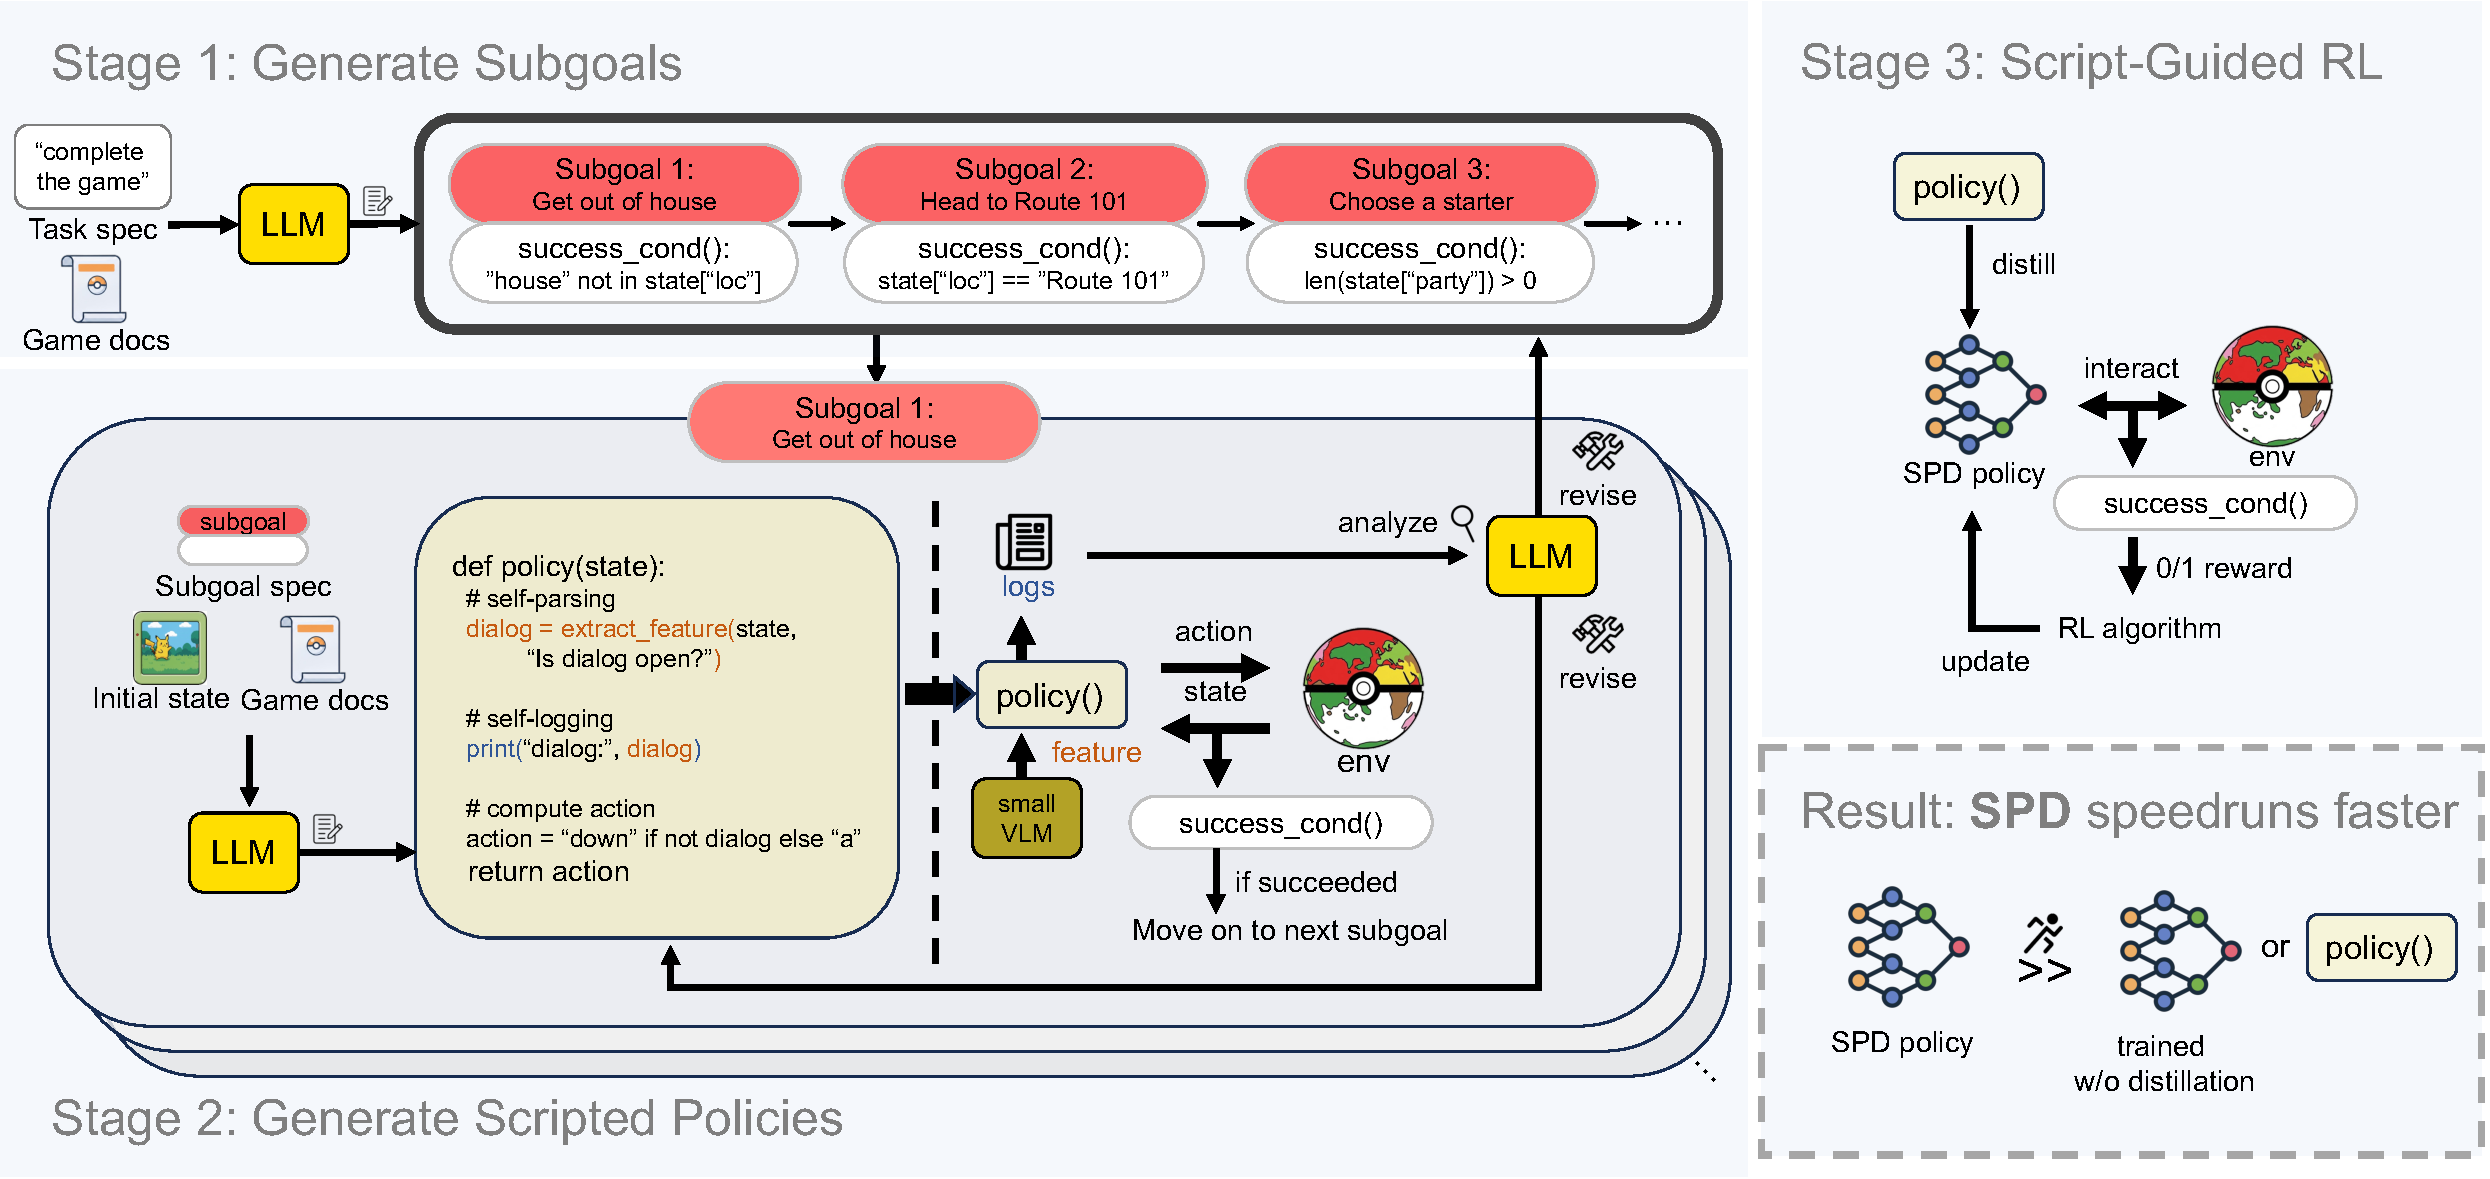
\includegraphics[width=\textwidth]{appendix_competitors/heatz_figure.pdf}
  \caption{\textbf{Overview of Scripted Policy Distillation (SPD).} The approach consists of three stages: (1) Subgoal Generation where an LLM decomposes the task into sequential subgoals with executable success conditions; (2) Scripted Policy Generation where the LLM generates policies that can invoke VLM tools and use self-directed logging for debugging; (3) Script-Guided RL where scripted policies are distilled into neural networks via supervised learning followed by RL with expert action guidance.}
  \label{fig:heatz_method}
\end{figure}

Reinforcement learning offers a powerful framework for training autonomous agents, yet applying RL directly to long-horizon tasks with sparse rewards remains fundamentally challenging. To address this, Heatz proposed leveraging LLM-generated scripted policies as priors for RL exploration (Figure~\ref{fig:heatz_method}). Although these scripted policies are not always optimal, they facilitate RL training by initializing exploration from a distribution that already reaches the goal, rather than from scratch. The framework, \textbf{Scripted Policy Distillation (SPD)}, consists of three stages: (1) subgoal generation, (2) scripted policy generation, and (3) script-guided RL.

\paragraph{Subgoal generation.} Given a long-horizon task specification, an LLM decomposes the task into a sequence of subgoals, each paired with an executable success-condition function \texttt{success\_cond(state)} that determines subgoal completion.

\paragraph{Scripted policy generation.} For each subgoal, the LLM generates a scripted policy that maps states to actions. The scripted policy interacts with the environment until \texttt{success\_cond(state)} returns \texttt{True} or a timeout occurs. Upon failure, the LLM analyzes execution traces and revises either the policy code or the subgoal specification. Policies can optionally query a vision-language model (Qwen3-VL-8B) for visual cues, and self-directed logging provides concise summaries of agent interactions rather than full execution trajectories.

\paragraph{Script-guided RL.} Once all scripted policies reliably achieve their subgoals, they are distilled into neural network policies via imitation learning on expert trajectories, followed by RL with expert action guidance. A DQN agent is trained with expert trajectories seeded into the replay buffer and expert actions executed with annealed probability during rollouts.

SPD achieved a 40:13 completion time. The resulting policy exhibited emergent behaviors: BFS-based local pathfinding during scripted policy generation, and after distillation, shorter routes, trainer battle skipping, and faster menu interactions discovered through RL optimization.

\subsection{Hamburg Pok\'{e}Runners (Second Place)}\label{sec:hamburg}

\textbf{Team:} Benedikt Schink, Arian Urdu, Matin Urdu

\begin{figure}[h]
    \centering
    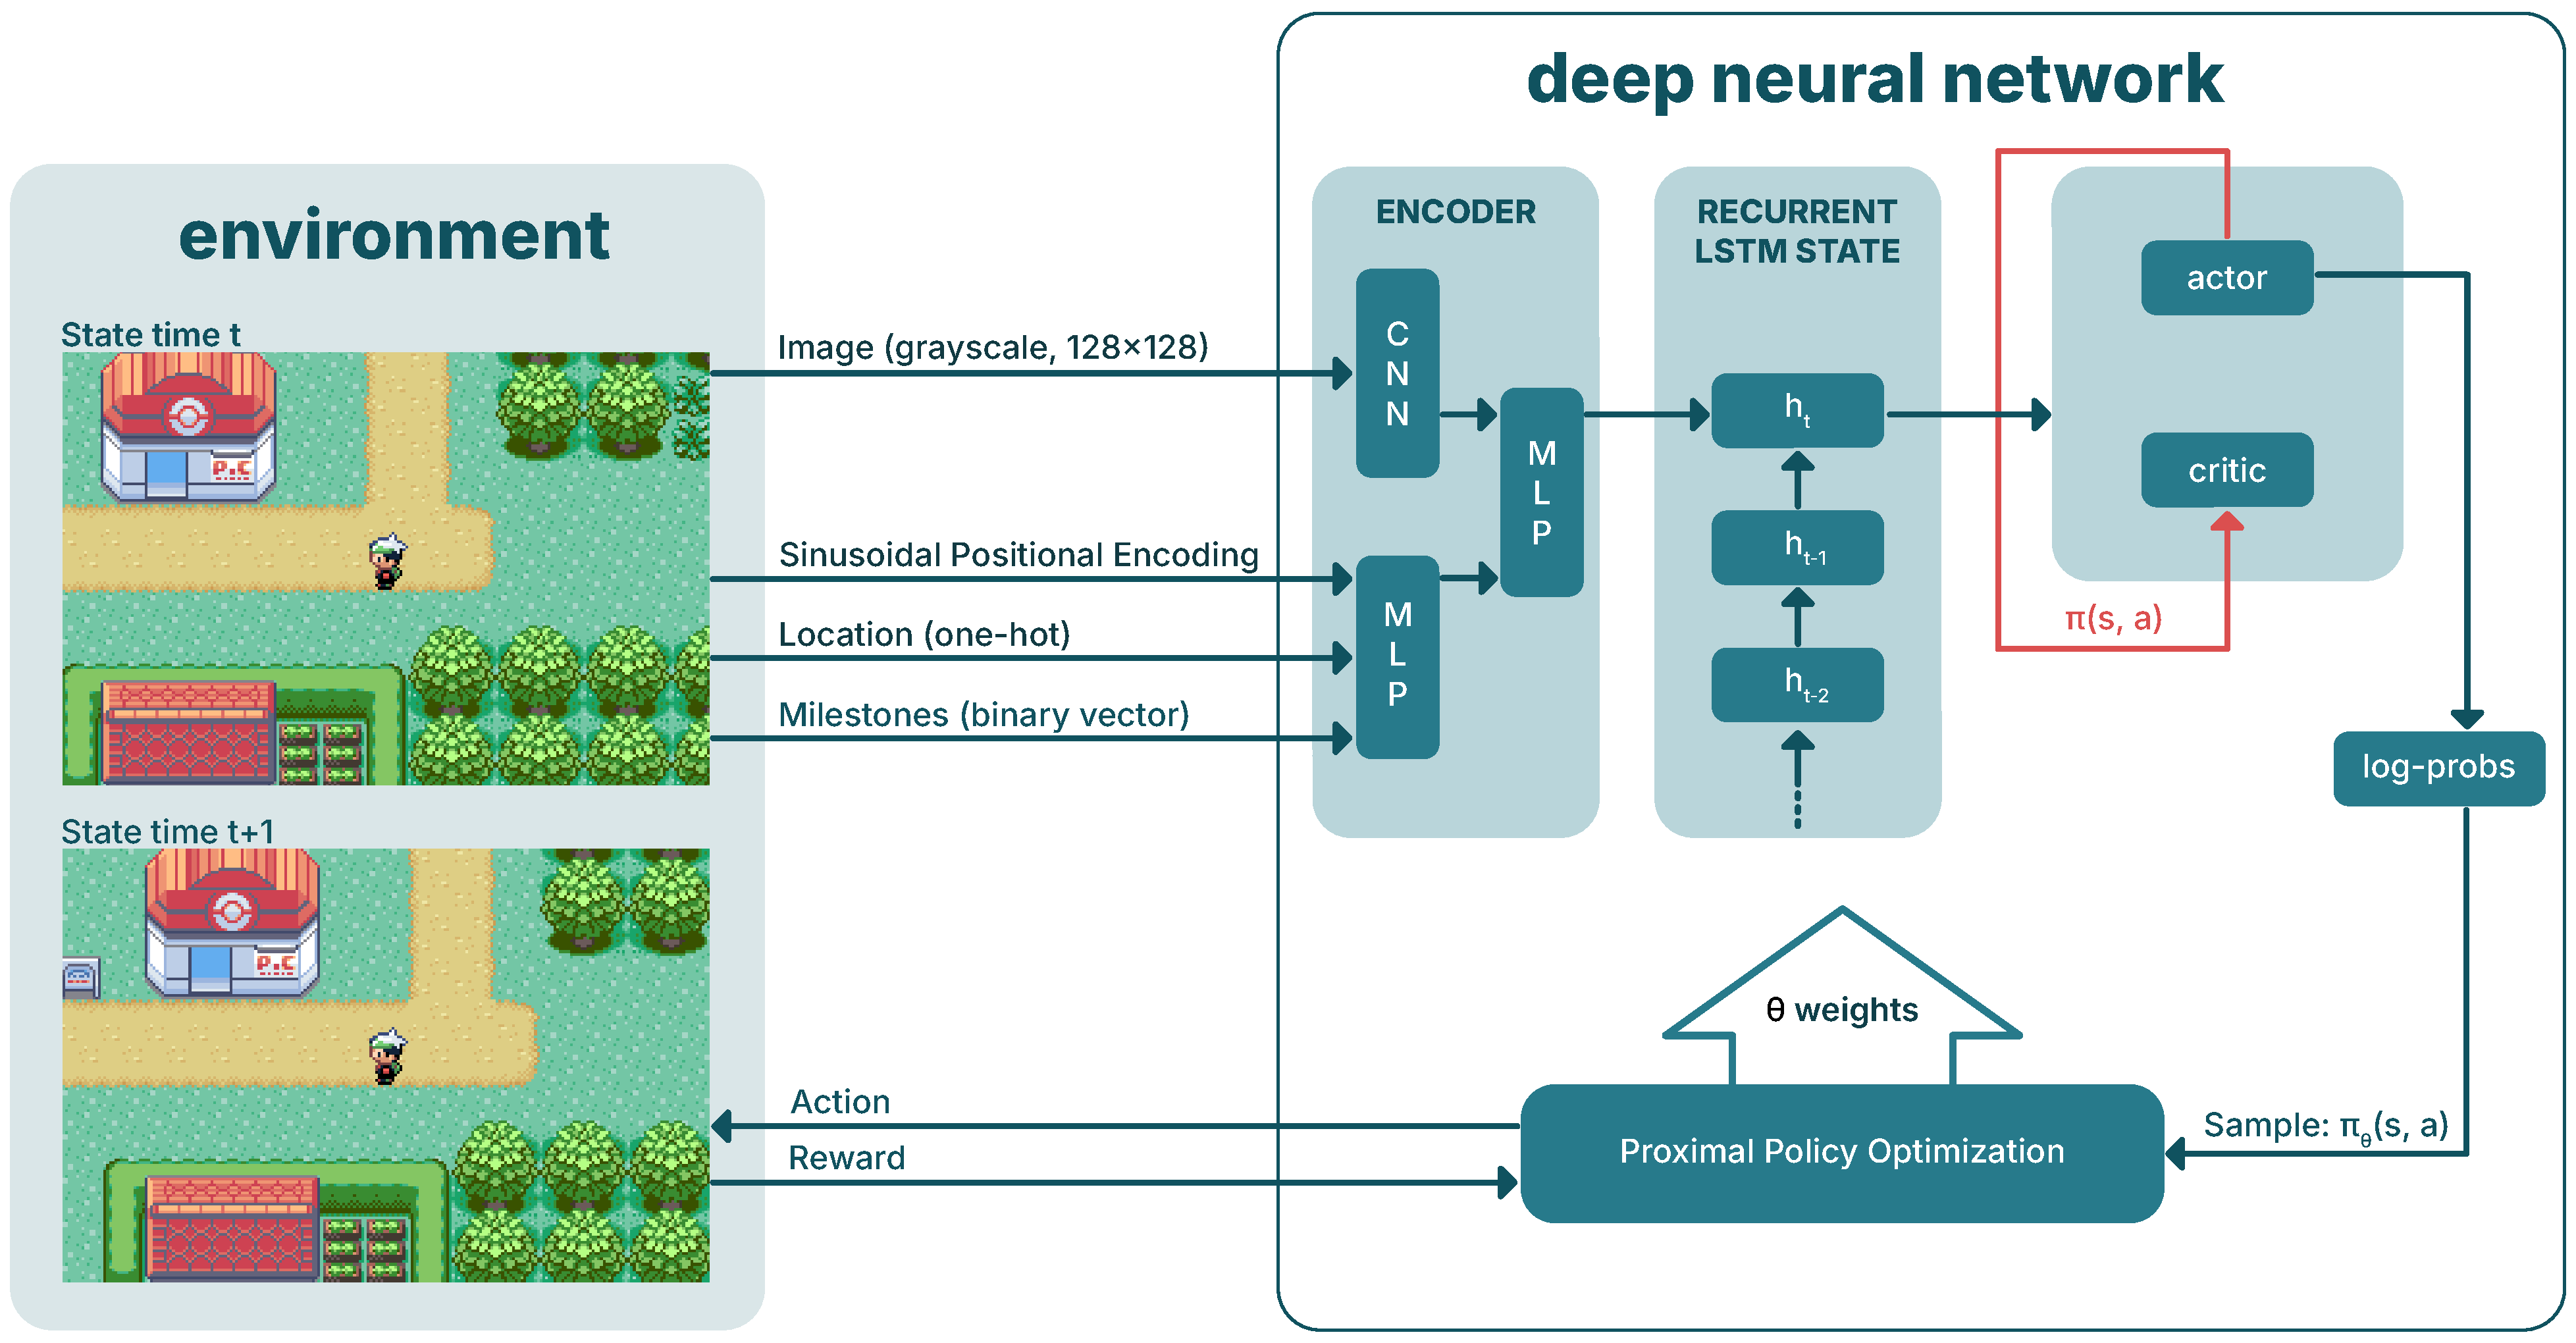
\includegraphics[width=0.8\textwidth]{appendix_competitors/hamburg_architecture.pdf}
    \caption{Hamburg Pok\'{e}Runners' recurrent PPO architecture, showing the CNN encoder for visual input, MLP for positional and milestone encoding, and LSTM for temporal reasoning.}
    \label{fig:hamburg_architecture}
\end{figure}

Hamburg Pok\'{e}Runners achieved second place (first badge: 01:14:43) using a reinforcement learning approach based on recurrent proximal policy optimization (PPO). The architecture consists of a CNN encoder receiving downsampled game frames (grayscale, $128 \times 128$ pixels), sinusoidal positional encodings for in-game coordinates, one-hot location encoding, and a binary milestone vector $m \in \{0, 1\}^{38}$ encoding sub-milestones and visited locations. An LSTM in the recurrent state provides temporal reasoning (Figure~\ref{fig:hamburg_architecture}).

The milestone vector played a crucial role in stability: it served both as a memory component (tracking achievements) and as goal conditioning (tracking the current objective), making the model more robust to the inherent randomness of Pok\'{e}mon Emerald and non-deterministic input/output latency. The team observed simple error-correcting behavior where the agent would overshoot or undershoot targets and backtrack to correct its trajectory.

The reward function includes only positive rewards: competition sub-milestones, locations visited, coordinate exploration, badges, money earned, HP healed, Pok\'{e}mon leveled, and damaging attacks used. All negative rewards (e.g., step penalties) caused model degradation as the agent reverted to safe, non-progressive behavior. Due to limited computational resources, multiple smaller models were trained and stitched together during inference.

\subsection{Anthonys (Third Place)}\label{sec:anthonys}

\textbf{Author:} Anthony Sistilli

Anthonys' approach centered on decomposing game progression into discrete phases with specialized navigation strategies for each context. The core innovation was combining deterministic pathfinding algorithms with context-aware prompt engineering.

\textbf{Phase-Based State Management}: The challenge was structured into seven distinct phases corresponding to major game milestones. Each phase maintained its own prompt template with conditional instructions that dynamically adapted based on completed objectives and current location.

\textbf{A* Pathfinding with Directional Priorities}: Rather than relying solely on the LLM for spatial reasoning, A* pathfinding was implemented on the game map grid to compute optimal movement sequences. The system extracted walkable tiles from game memory, constructed a navigable grid, and generated action sequences to reach target coordinates.

\textbf{Battle State Management}: Battle sequences required special handling due to the game's menu system complexity. An input-clearing mechanism sent predetermined button sequences to ensure the agent escaped bad states.

\textbf{Adaptive Recovery and Stuck Detection}: The system tracked position history to detect when the agent remained stationary for multiple turns, indicating an obstacle or navigation failure.

\subsection{Deepest (Judge's Choice: Most Efficient)}\label{sec:deepest}

\textbf{Team:} Seonghun Hong, Hyunyoung Jeong, Hyeokgi Kim, Jaeyoon Jung \\
\textbf{Affiliation:} Seoul National University, Soongsil University, MAUM.AI

\begin{figure}[h]
    \centering
    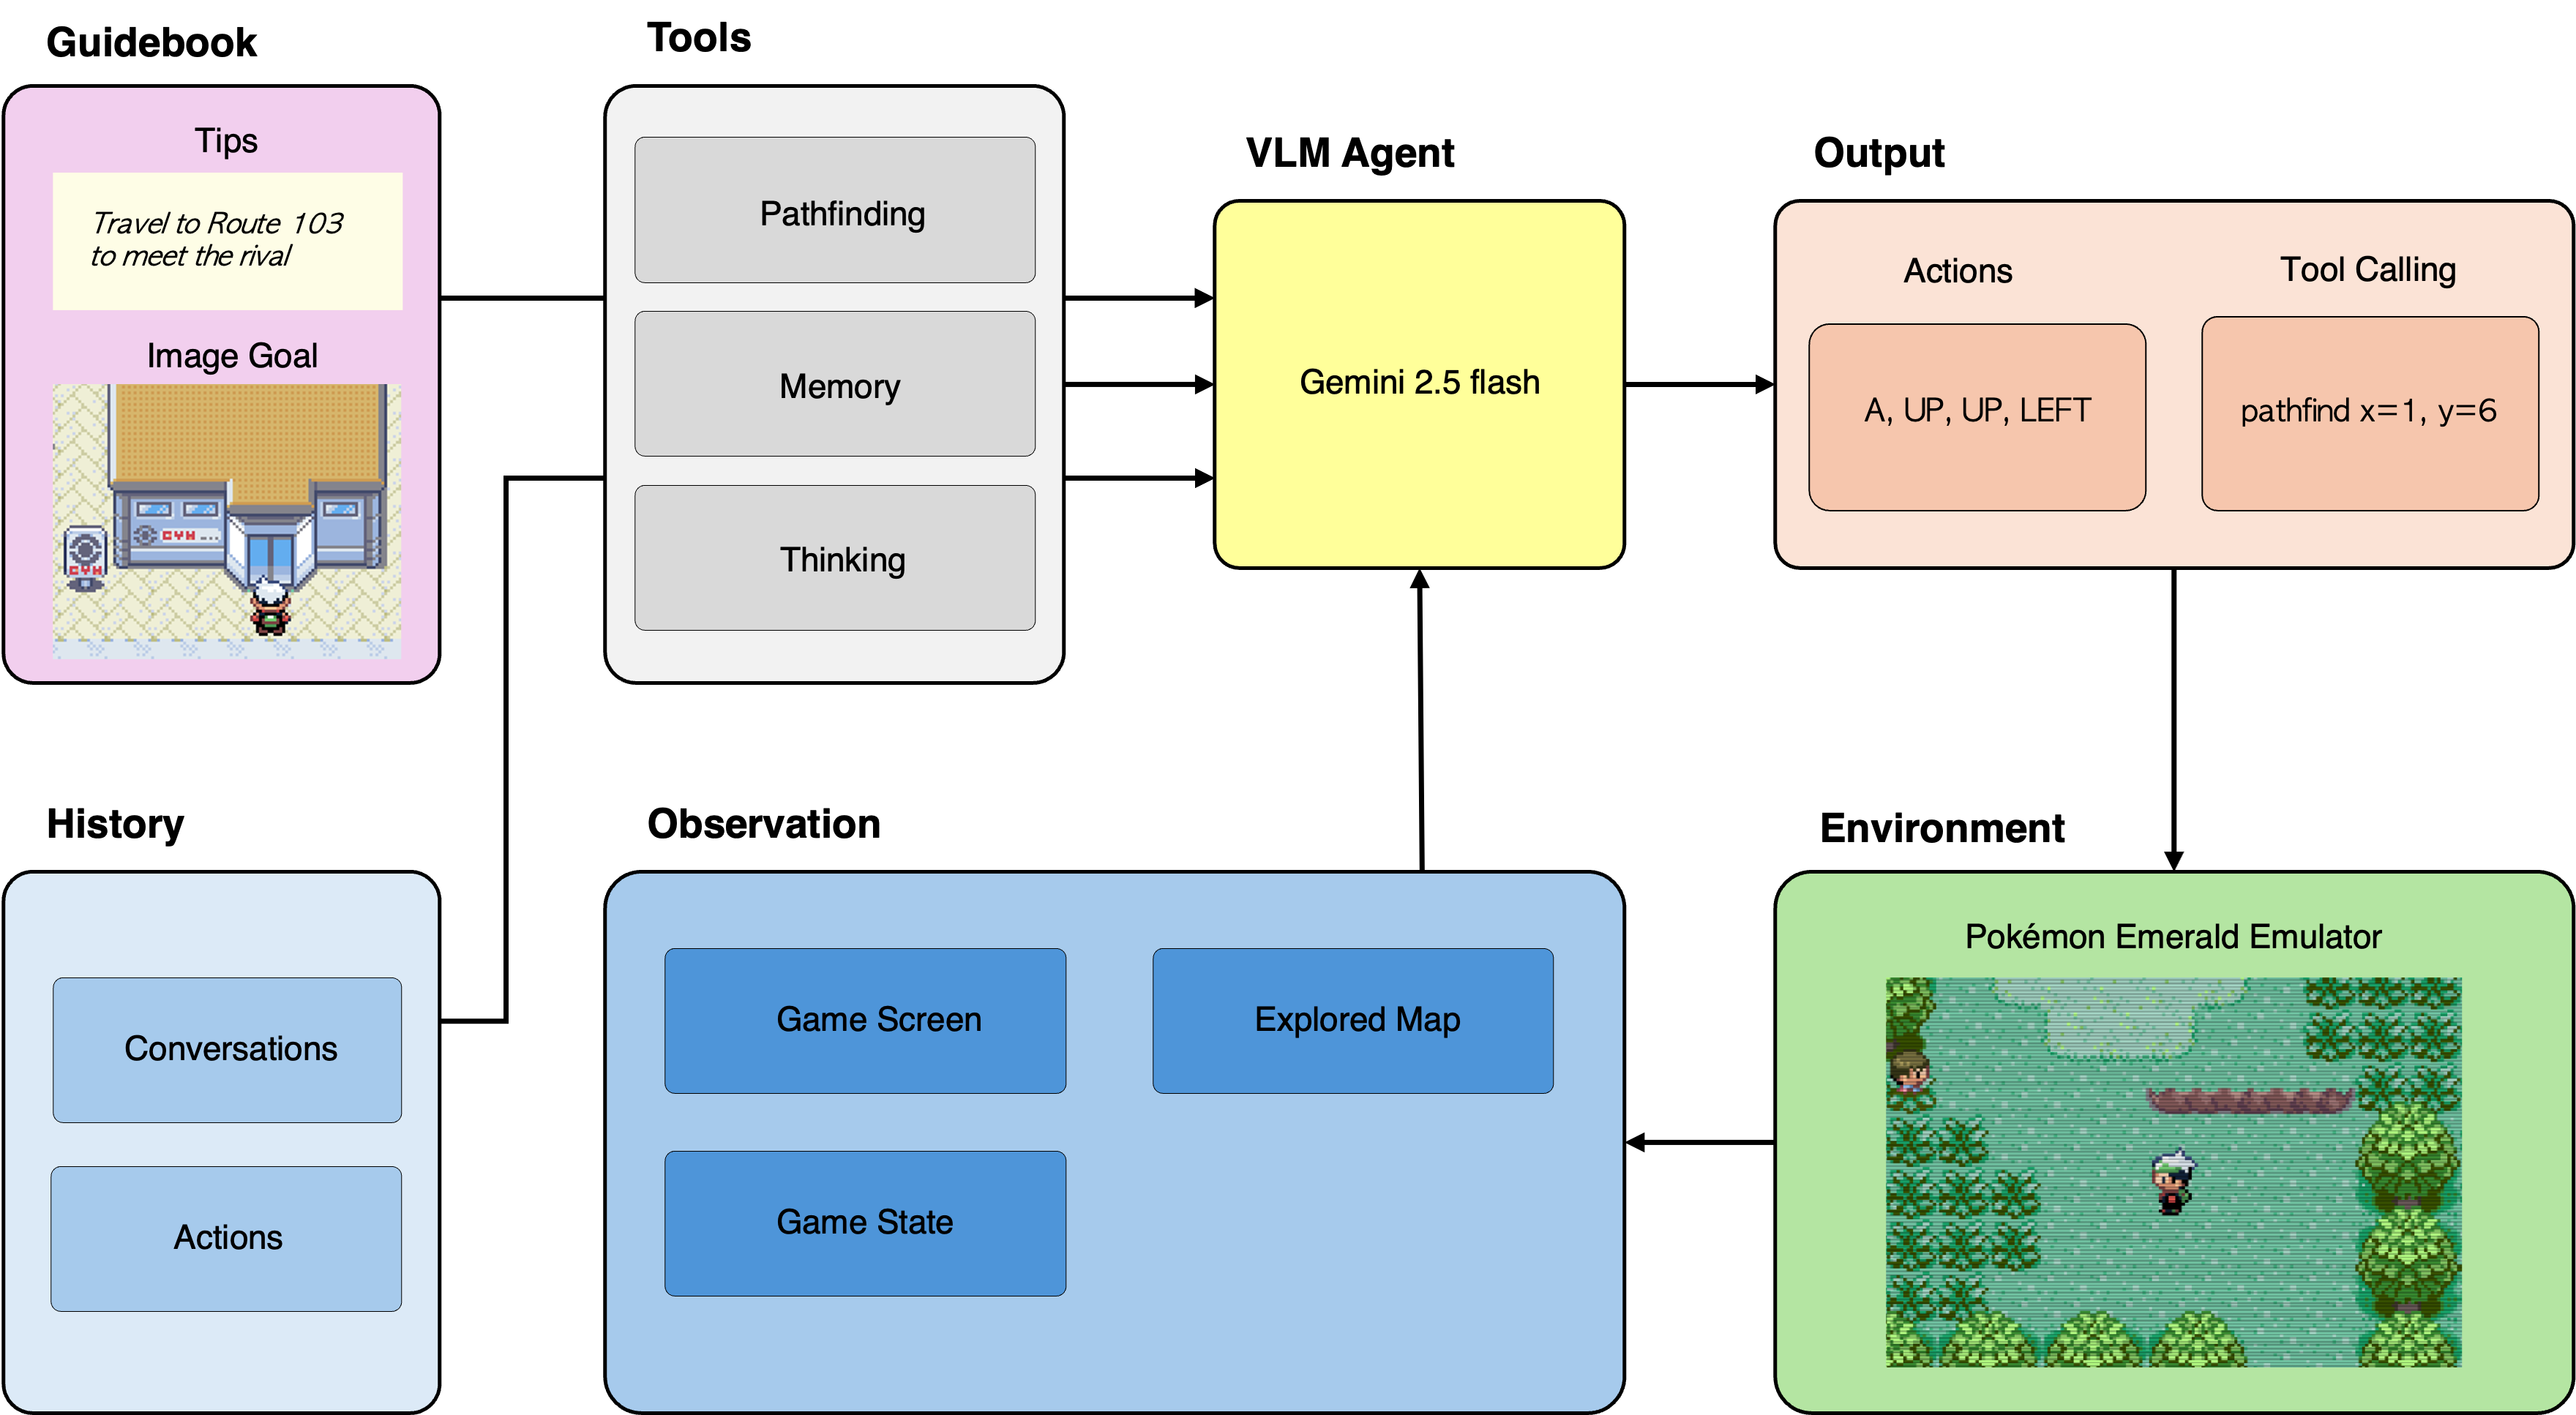
\includegraphics[width=0.92\textwidth]{appendix_competitors/deepest_architecture.png}
    \caption{Deepest agent architecture. The agent receives partial observations and milestone-specific guidance from the Guidebook. Gemini 2.5 Flash reasons and outputs actions, optionally invoking tools (Pathfinding, Memory, Thinking). Actions execute in the emulator, producing the next observation.}
    \label{fig:deepest_architecture}
\end{figure}

Deepest proposed a training-free, fully autonomous agent architecture that operates under human-like perceptual constraints using Gemini 2.5 Flash. The approach achieved 5th place by time (02:04:29) but received the Judge's Award for most sample-efficient completion, completing in just 649 actions---the fewest of any team (Figure~\ref{fig:deepest_architecture}).

A core design principle is the absence of privileged game state: the agent receives no ground-truth map information, and all navigation decisions are computed exclusively from partially observed tiles explored during gameplay. To support high-level strategy, a \textbf{Guidebook} system provides milestone-specific knowledge (e.g., selecting Mudkip for type advantage). \textbf{Image goals}---reference images of destination locations---enable the agent to visually recognize objectives.

Three auxiliary tools augment the agent's capabilities:
\begin{itemize}[nosep]
    \item \textbf{Pathfinding Tool}: coordinate-based navigation for known destinations and directional exploration for unknown ones, using A* on the observed map grid with game-specific constraints.
    \item \textbf{Memory Tool}: explicit persistence of critical state information with a sliding window policy retaining memory over the most recent 10 conversation turns.
    \item \textbf{Thinking Tool}: adaptive computation toggling the model's reasoning budget---2048 tokens for complex decisions, 512 for routine navigation.
\end{itemize}

\section{Expert Harness Tool Reference}\label{sec:appendix_tools}

This section provides a complete reference for the MCP tools and subagent tool access configurations in $\mathcal{H}_{\text{expert}}$ as described in Section~\ref{sec:system_design}.

\subsection{Tool Access by Agent Role}\label{sec:appendix_tool_access}

Table~\ref{tab:tool_access} details which tools are available to each agent role within the expert harness. The orchestrator has the broadest access; subagents receive restricted tool sets to enforce separation of concerns. Tools marked with $\dagger$ are available only in $\mathcal{H}_{\text{expert}}$ (stripped in $\mathcal{H}_{\min}$ and $\mathcal{H}_{\text{auto}}$). Custom subagents receive a configurable tool set specified at creation time, subject to the constraint that \texttt{execute\_custom\_subagent} is always forbidden (no recursive subagent spawning).

\begin{table}[h]
\centering
\caption{Tool access matrix by agent role. \cmark{} = available, \xmark{} = unavailable, $\dagger$ = $\mathcal{H}_{\text{expert}}$ only.}
\label{tab:tool_access}
\small
\begin{tabular}{l c c c c}
\toprule
\textbf{Tool} & \textbf{Orchestrator} & \textbf{Battler} & \textbf{Planner} & \textbf{1-Step} \\
\midrule
\multicolumn{5}{l}{\textit{Game Control}} \\
\texttt{press\_buttons}           & \cmark & \cmark & \xmark & \xmark \\
\texttt{complete\_direct\_objective} & \cmark & \xmark & \xmark & \xmark \\
\texttt{navigate\_to}$^\dagger$   & \cmark & \xmark & \xmark & \xmark \\
\midrule
\multicolumn{5}{l}{\textit{Memory}} \\
\texttt{process\_memory}          & \cmark & \cmark & \cmark & \xmark \\
\texttt{add\_memory}              & \xmark & \cmark & \cmark & \xmark \\
\texttt{search\_memory}           & \xmark & \cmark & \cmark & \xmark \\
\texttt{get\_memory\_summary}     & \xmark & \cmark & \cmark & \xmark \\
\midrule
\multicolumn{5}{l}{\textit{Skills \& Code Execution}} \\
\texttt{process\_skill}           & \cmark & \cmark & \cmark & \xmark \\
\texttt{run\_skill}               & \cmark & \xmark & \xmark & \xmark \\
\texttt{run\_code}                & \cmark & \xmark & \xmark & \xmark \\
\midrule
\multicolumn{5}{l}{\textit{Research \& Planning}} \\
\texttt{get\_progress\_summary}$^\dagger$ & \cmark & \cmark & \cmark & \xmark \\
\texttt{get\_walkthrough}$^\dagger$ & \cmark & \xmark & \cmark & \xmark \\
\texttt{lookup\_pokemon\_info}$^\dagger$ & \cmark & \cmark & \cmark & \xmark \\
\texttt{replan\_objectives}       & \xmark & \xmark & \cmark & \xmark \\
\midrule
\multicolumn{5}{l}{\textit{Subagent Management}} \\
\texttt{process\_subagent}        & \cmark & \xmark & \xmark & \xmark \\
\texttt{execute\_custom\_subagent} & \cmark & \xmark & \xmark & \xmark \\
\bottomrule
\end{tabular}
\vspace{0.5em}

\footnotesize{1-step subagents (\texttt{reflect}, \texttt{verify}, \texttt{summarize}, \texttt{gym\_puzzle}) receive no tool access; they perform a single VLM pass over a trajectory window segment. The planner additionally has access to the four built-in 1-step subagents and \texttt{replan\_objectives} for objective CRUD operations.}
\end{table}

\subsection{MCP Tool Definitions}\label{sec:appendix_tool_defs}

Table~\ref{tab:tool_defs} provides brief descriptions of all MCP tools exposed by the game server, plus locally defined tools in the agent process.

\begin{table}[h]
\centering
\caption{Complete MCP tool reference for the \pokeagent{} harness.}
\label{tab:tool_defs}
\small
\begin{tabular}{l p{9.5cm}}
\toprule
\textbf{Tool} & \textbf{Description} \\
\midrule
\multicolumn{2}{l}{\textit{Game Control}} \\
\texttt{get\_game\_state}        & Returns current observation: screenshot, ASCII map, party, bag, location, coordinates, and game context (overworld/battle/dialog/menu). Called automatically each step. \\
\texttt{press\_buttons}          & Executes a sequence of GBA button presses (\texttt{A}, \texttt{B}, directional, \texttt{START}, \texttt{SELECT}, \texttt{L}, \texttt{R}, \texttt{WAIT}). \\
\texttt{complete\_direct\_objective} & Marks the current direct objective as completed and advances to the next in the specified category (story, battling, or dynamics). \\
\texttt{navigate\_to}            & A* pathfinding to target $(x,y)$ coordinates with configurable path variance and NPC collision avoidance. \\
\midrule
\multicolumn{2}{l}{\textit{Persistent Memory (CRUD)}} \\
\texttt{process\_memory}         & Unified CRUD for hierarchical long-term memory entries (read, add, update, delete). \\
\texttt{add\_memory}             & Add a single entry to the long-term memory store (legacy interface). \\
\texttt{search\_memory}          & Keyword search over long-term memory entries. \\
\texttt{get\_memory\_summary}    & Retrieve a summary of the long-term memory store. \\
\texttt{get\_memory\_overview}   & Compact tree view of all memory entry IDs and titles. \\
\midrule
\multicolumn{2}{l}{\textit{Skill Library}} \\
\texttt{process\_skill}          & Unified CRUD for skill library entries (behavioral or executable). \\
\texttt{get\_skill\_overview}    & Compact tree view of all skill IDs and names. \\
\texttt{run\_skill}              & Execute a skill's Python code in the sandbox with game tool access. \\
\texttt{run\_code}               & Execute arbitrary Python in the sandbox (read-only game tools) for prototyping. \\
\midrule
\multicolumn{2}{l}{\textit{Subagent Registry}} \\
\texttt{process\_subagent}       & Unified CRUD for the subagent registry (create, inspect, update, delete entries). \\
\texttt{get\_subagent\_overview} & Compact tree view of all subagent IDs and names. \\
\midrule
\multicolumn{2}{l}{\textit{Research \& Progress}} \\
\texttt{get\_progress\_summary}  & Milestones, location, objective status, completed objectives, and memory overview. \\
\texttt{get\_walkthrough}        & Retrieve a section of the Pok\'{e}mon Emerald walkthrough (Parts 1--21). \\
\texttt{lookup\_pokemon\_info}   & Query Bulbapedia for Pok\'{e}mon stats, moves, evolution, and location data. \\
\texttt{list\_wiki\_sources}     & List available wiki data sources for \texttt{lookup\_pokemon\_info}. \\
\midrule
\multicolumn{2}{l}{\textit{Objective Management}} \\
\texttt{get\_full\_objective\_sequence} & Return the complete objective state across all categories. \\
\texttt{replan\_objectives}      & Apply index-based edits (add, complete, reorder, delete) to objectives within a single category. \\
\midrule
\multicolumn{2}{l}{\textit{Spatial Memory (Experimental)}} \\
\texttt{save\_map}               & Save the agent's mental map of a location to persistent storage. \\
\texttt{load\_map}               & Load a previously saved mental map for a location. \\
\bottomrule
\end{tabular}
\end{table}

\section{Example Prompts for Ablation Studies}\label{sec:appendix_prompts}

\textit{[To be written. Representative system prompts, base prompts, and evolution outputs across experimental conditions.]}

\section{Gameplay Demonstrations}\label{sec:appendix_gameplay}

\textit{[To be written. Selected trajectory excerpts illustrating agent behavior across different harness configurations. Annotated reasoning traces.]}

\section{AutoEvolve Store Comparisons}\label{sec:appendix_stores}

\textit{[To be written. Full memory, skill, and subagent store snapshots across AutoEvolve experiments, comparing evolved artifacts across trials and settings.]}

\section{Engineering Standards}\label{sec:appendix_engineering_standards}

Per the ECE Department's Independent Work and Thesis Handbook, this section identifies the engineering standards and broadly accepted industrial conventions used in this thesis.

\textit{[To be completed. The following categories should be addressed with specific standards, tools, and their role in the project:]}

\begin{itemize}
    \item \textbf{Software frameworks and libraries.} \textit{[e.g., Python 3.x, FastAPI, mGBA emulator SDK, Google Generative AI SDK, NumPy. Describe role of each in the system.]}
    \item \textbf{Communication protocols.} \textit{[e.g., HTTP/REST for agent--server communication, WebSocket for frame streaming, Model Context Protocol (MCP) for tool integration. Cite relevant specifications.]}
    \item \textbf{Data formats and serialization.} \textit{[e.g., JSON for structured state representation and tool call/response payloads, PNG for frame capture, BibTeX for bibliography management.]}
    \item \textbf{Evaluation methodology.} \textit{[e.g., wall-clock timing standards, milestone-based progress metrics, token counting conventions, cost estimation methodology.]}
    \item \textbf{Reproducibility and open-source practices.} \textit{[e.g., version control (Git), open-source licensing, public benchmark release, documentation standards.]}
    \item \textbf{Security and sandboxing.} \textit{[e.g., restricted built-in functions in the code execution sandbox, process-local isolation for agent-generated code.]}
    \item \textbf{Game emulation.} \textit{[e.g., mGBA emulator accuracy standards, GBA hardware specifications ($240 \times 160$ resolution, ARM7TDMI processor), ROM integrity verification.]}
\end{itemize}


\end{document}
